\documentclass{pnastwo}
%\documentclass[10pt,twocolumn]{article}


%\usepackage[margin=1in]{geometry}
%\usepackage{graphicx}
\graphicspath{ {paper_figures2/} }

\usepackage{tikz}

\usepackage{float}
\usepackage{amssymb,amsfonts,amsmath}
\DeclareMathOperator*{\argmin}{arg\,min}

\makeatletter
\newcommand{\customlabel}[2]{%
\protected@write \@auxout {}{\string \newlabel {#1}{{#2}{}}}}
\makeatother

\renewcommand\thefigure{S\arabic{figure}}    

\newcommand{\fig}[0]{Fig.}

\begin{document}



\begin{article}


\section{Materials and Methods}

\subsection{Measuring developmental time during cellularization}


\begin{itemize}
\item We need to have a supplementary figure that shows the lateral view, that makes it even more clear that we work with optical sections.

\item Need image labeled with D/V

\end{itemize}




\subsection{Image parameters}

Each image is subsampled to $100 \times 100$ pixels.
%
For the first and third data sets in the paper (images taken during cellularization), we only use the red and green channels (dpERK and Dl) in the vector diffusion maps computations, as the spatial location of the nuclei does not change appreciably during this time window.
%
The nuclei in the corresponding figures are shown only for visual reference.
%
For the second data set of images during gastrulation, we use all three channels (dpERK, Twi, and nuclei) in the vector diffusion maps computations.
%
We blur the nuclear signal using a disc filter with a $5$~pixel radius (using the \texttt{imfilter} function in Matlab with a disc filter).
%
We also adjust the intensity of the nuclear signal in each image such that 1\% of the pixels are saturated (using the \texttt{imadjust} function in Matlab).

When imaging, the laser settings were calibrated so that images have good dynamic range, while not saturating the detector. 
% 
The same laser setting is maintained within each experiment. 

{\bf discuss how we choose weights of signals}



\subsection{Mathematical Algorithms}

We will demonstrate the algorithms for registration and temporal ordering using a synthetic data set.
%
The relatively simple dynamics of this data set will allow us to easily visualize and illustrate the main points of the different algorithms.
%
We construct concentration profiles defined on a ring, and we assume that each ring is arbitrarily rotated around its center; an example is shown in \fig~\ref{subfig:1d_example}.
%
Rotation of the ring corresponds to shifting (with periodic boundary conditions) the one-dimensional concentration profile shown at the bottom of \fig~\ref{subfig:1d_example} (the symmetry group is $SO(2)$, the group of all two-dimensional proper rotations).
%
Each concentration profile is a noisy Gaussian (shown in \fig~\ref{subfig:1d_intensity}), and the Gaussians increase in intensity as  a function of time.
%
We discretize the profiles into $100$ points, so our numerical data will be $100$-dimensional vectors (the corresponding symmetry group for the discretized profiles is $\mathbb{Z}_{100}$, the group of integers modulo $100$).
%
\fig~\ref{subfig:1d_unaligned_unordered} shows the entire data set; the concentration profiles have been stacked in an array, so that each row corresponds to a single profile.
%
Because the profiles are unregistered and unordered, the underlying dynamics (a Gaussian whose amplitude grows in time) are not readily apparent.



\subsubsection{Angular synchronization \cite{singer2011angular}}

Let $ x_1, \dots, x_m$ denote the signals that we wish to align with respect to rotations;
each signal is a function defined on the unit circle (on the plane).
%
%Practically, it is discretized in a $n$-long vector (the local intensity at $n$ equidistant points around the circle);
%rotating the function by an angle $\theta$ then corresponds to cyclically shifting the elements of $x_i$ by $\frac{\theta_i}{2 \pi} n$ (rounded to the nearest integer to obtain a valid shift).
%
First assume that each signal $x_i$ is a {\it noisy} rotated copy of the underlying signal $x_{true}$
(which we are {\it not} given), such that
\begin{equation}
x_i = f(x_{true}, \theta_i) + \xi_i
\end{equation}
where the function $f(x_{true}, \theta_i)$ rotates the signal $x_{true}$ by $\theta_i$ radians, and $\xi_i$ is a (typically Gaussian) noise term.
%
Our goal is to recover $\theta_1, \dots, \theta_m$.
%
Up to noise,
\begin{equation} \label{eq:pairwise_rot}
x_i \approx f(x_j, \theta_i - \theta_j) ;
\end{equation}
note that \eqref{eq:pairwise_rot} does not require knowledge of $x_{true}$.
%
We can obtain an {\it estimate} of $\theta_i - \theta_j$ by computing the rotation that optimally aligns $x_j$ to $x_i$,
i.e., %$\theta_{ij} \approx \theta_i - \theta_j$, where
%
\begin{equation} \label{eq:opt_angle}
\theta_i - \theta_j \approx \theta_{ij} = \argmin_{\theta} \|x_i - f(x_j, \theta)\|^2.
\end{equation}
%
Practically, the signals are discretized in a $n$-long vector (the local intensity at $n$ equidistant points around the circle);
rotating the function by an angle $\theta$ then corresponds to cyclically shifting the elements of $x_i$
by $\frac{\theta_i}{2 \pi} n$ (rounded to the nearest integer to obtain a valid shift).
%
For the one-dimensional discretized profiles shown in \fig~\ref{fig:1d_demo}, we exhaustively search over all $n=100$ possible shifts of the signals to compute the optimal angles in \eqref{eq:opt_angle}.
%
Alternatively, for continuous signals, an optimization algorithm
can be used \cite{ahuja2007template}.

Rather than work with the angles $\theta_{ij}$ directly, it is more convenient to consider the	 rotation matrices,
\begin{equation} \label{eq:R_theta}
R(\theta_{ij}) = \begin{bmatrix}
\cos(\theta_{ij}) & -\sin(\theta_{ij}) \\
\sin(\theta_{ij}) & \cos(\theta_{ij})
\end{bmatrix},
\end{equation}
which we can think of as operating on the points of the unit circle (on the plane) on which our signal is defined.
%
Successive rotations correspond to multiplication of the corresponding rotation matrices: $R(\alpha_1 + \alpha_2) = R(\alpha_1) R(\alpha_2)$.
%
Due to the orthogonality of rotation matrices, $R(-\alpha) = R(\alpha)^T$.

Let $d$ denote the dimension of the rotation matrices we are considering (for our example of planar rotations, $R(\theta_{ij}) \in \mathbb{R}^{2 \times 2}$ and $d=2$; we write our procedure for general $d$ because we will later consider three-dimensional rotations).
%
We construct the matrix $H \in \mathbb{R}^{md \times md}$, where $H$ is an $m \times m$ matrix of $d \times d$ blocks, with the $i,j^{th}$ block of $H$, $H_{ij}$, defined as
\begin{equation} \label{eq:H_to_R}
H_{ij} = R(\theta_{ij}).
\end{equation}
%
%
Under our assumption that $\theta_{ij} \approx \theta_i - \theta_j$, $H_{ij} \approx R(\theta_i) R(\theta_j)^T$
%\begin{equation}
%H_{ij} = R(\theta_{ij}) \approx R(\theta_i - \theta_j) = R(\theta_i) R(-\theta_j) = R(\theta_i) R(\theta_j)^T,
%\end{equation}
 and
\begin{equation} \label{eq:H_low_rank}
	H \approx
	\begin{bmatrix}
	R(\theta_1) \\
	R(\theta_2) \\
	\vdots \\
	R(\theta_m)
	\end{bmatrix}
	\begin{bmatrix}
	R(\theta_1)^T R(\theta_2)^T \dots R(\theta_m)^T
	\end{bmatrix}.
\end{equation}
%
It follows directly from \eqref{eq:H_low_rank} that the top block eigenvector of $H$ contains our best estimates of $R(\theta_1), R(\theta_2), \dots, R(\theta_m)$.
%
Let $\phi_1, \phi_2, \dots, \phi_{md}$ denote the eigenvectors of $H$, ordered such that $|\lambda_1| \ge |\lambda_2| \ge \dots \ge |\lambda_{md}|$, where $\lambda_i$ is the eigenvalue corresponding to $\phi_i$.
%
Then,
\begin{equation} \label{eq:R_hat}
\hat{R} =
\begin{bmatrix}
\hat{R}_1 \\
\hat{R}_2 \\
\vdots \\
\hat{R}_m
\end{bmatrix} =
\begin{bmatrix}
| & | & & | \\
\phi_1 & \phi_2 & \dots & \phi_d \\
| & | & & |
\end{bmatrix},
\end{equation}
where $\hat{R}_i \in \mathbb{R}^{d \times d}$ is (nearly) the estimate for $R(\theta_i)$.
%
To obtain our estimate of $R(\theta_i$), denoted $R_{i, est}$, we project $\hat{R}_i$ onto the closest orthogonal matrix, 
\begin{equation} \label{eq:R_est}
R_{i, est} = U_i V_i^T,
\end{equation}
where $U_i$ and $V_i$ are the left and right singular vectors, respectively, of $\hat{R}_i$.
%
We adjust the sign of $\phi_1$ so that $det(R_{i, est}) = +1$, ensuring proper rotations.
%
We estimate $\theta_{i}$ by inverting \eqref{eq:R_theta}, and register the signals by rotating signal $i$ by $-\theta_i$.
%
We note that, in our actual computations, the pairwise rotations $\theta_{ij}$ are computed in a discrete setting, then the overall
synchronization is performed in the continuum context to obtain $\theta_i$, and the results are rounded to give the closest
discrete shift.

Furthermore, this formulation also considers {\it higher-order} consistency information.
%
For example, given our pairwise estimates $R_{ij}$, we know that relationships of the form
\begin{equation} \label{eq:triplet_consistency}
R(\theta_{ik}) R(\theta_{kj}) \approx R(\theta_i) R(\theta_k)^T R(\theta_k) R(\theta_j)^T = R(\theta_i) R(\theta_j)^T
\end{equation}
should also hold.
%
Note that
\begin{equation}
(H^2)_{ij} = \sum_k R(\theta_{ik}) R(\theta_{kj});
\end{equation}
therefore, {\it all} information of the form in \eqref{eq:triplet_consistency} is contained in the matrix $H^2$.
%
Because $H$ and $H^2$ have the same eigenvectors, our problem formulation accounts for not only pairwise alignment information, but also these higher-order considerations.

\subsubsection{Diffusion maps \cite{coifman2005geometric}}

Given $m$ data points $x_1, \dots, x_m$ (typically vectors in a high-dimensional space), we want to find a coordinate transformation $y(x)$ that preserves local information: points that are close in the original space should also be close in the coordinate $y$.
%
The first step is to construct the matrix $W \in \mathbb{R}^{m \times m}$, where $W_{ij}$ is large if points $x_i$ and $x_j$ are ``close.''
%
We use a diffusion kernel,
\begin{equation} \label{eq:dmaps_W}
W_{ij} = \exp \left( -\frac{d^2(x_i, x_j)}{\epsilon^2} \right),
%W_{ij} = e^{ -\frac{d^2(x_i, x_j)}{\epsilon^2}}
\end{equation}
where $d(x_i, x_j)$ is a pairwise distance between $x_i$ and $x_j$ (often the Euclidean distance), and $\epsilon$ is a characteristic scale.
%
Points less than $\epsilon$ apart are thus considered ``close'' and points farther than $\epsilon$ apart are considered ``far away''.
%
$\epsilon$ can be chosen using several techniques (see, for example \cite{coifman2008graph, rohrdanz2011determination}); here, we take $\epsilon$ to be $1/10^{th}$ of the median of the pairwise distances between data points for the first two data sets, and half of the median of the pairwise distances between data points for the third data set.

To find this coordinate $y$, we want solve the following optimization problem \cite{Belkin2003}
\begin{equation} \label{eq:dmaps_opt_problem}
\argmin_{y} \sum_{ij} W_{ij} (y(x_i) - y(x_j))^2.
\end{equation}
%
We first compute the diagonal matrix $D$, where $D_{ii} = \sum_{j=1}^{m} W_{ij}$, and the matrix $A$, where
\begin{equation} \label{eq:dmaps_A}
A = D^{-1} W.
\end{equation}
%
We calculate the eigenvectors $\phi_1, \phi_2, \dots, \phi_m$, ordered such that $|\lambda_1| \ge |\lambda_2| \ge \dots \ge |\lambda_m|$.
%
Because the matrix $A$ is similar to the symmetric matrix $D^{-1/2} W D^{-1/2}$, $A$ is guaranteed to have real eigenvalues and real, orthogonal eigenvectors.
%
Because the matrix $A$ is row-stochastic, $\lambda_1=1$ and $\phi_1$ is a constant vector; this is a trivial solution to \eqref{eq:dmaps_opt_problem}.
%
%In general, the next few eigenvectors $\phi_2, \dots, \phi_m$ give ``meaningful'' embedding coordinates for the data, such that $\phi_j(i)$ gives the $j^{th}$ embedding coordinate of the $i^{th}$ data point.
%
The next eigenvector, $\phi_2$, is the (non-trivial) solution to \eqref{eq:dmaps_opt_problem}, so that $\phi_2(j)$, the $j^{th}$ entry of $\phi_2$, gives the ``new" coordinate for data point $x_j$ (i.e., $\phi_2(j) = y(x_j)$).
%
In our application, we have assumed that this single direction of variability, parameterized by $\phi_2$, is one-to-one with time.
%
Ordering the data by $\phi_2(j)$ will then, effectively, order them in time.
%
The procedure generalizes when the data lie on higher-dimensional manifolds (not just curves) in data space, where lower eigenvectors give subsequent embedding coordinates for the data.
%

\subsubsection{Vector diffusion maps\cite{singer2012vector}}

In vector diffusion maps, given data points $x_1, \dots, x_m$, one first constructs the matrix $S \in \mathbb{R}^{md \times md}$, with the $i,j^{th}$ block of $S$, $S_{ij}$, defined as
\begin{equation} \label{eq:vdm_S}
	S_{ij} = A_{ij} H_{ij}
\end{equation}
%
where $A_{ij} \in \mathbb{R}$ (defined in \eqref{eq:dmaps_A}) pertains to the diffusion kernel between data points, and $H_{ij} \in \mathbb{R}^{d \times d}$ (defined in \eqref{eq:H_to_R}) pertains to the pairwise alignment between data points.
%
It is important to note that distance $d(x_i, x_j)$ used in the diffusion kernel in \eqref{eq:dmaps_W} is the distance between data points {\it after} after pairwise alignment, i.e., the minimum distance between all possible shifts of the two data points (which is obtained in \eqref{eq:opt_pairwise}).
%
In the language of symmetry groups, this distance is a metric between the orbits induced by the symmetry group.

One then computes the eigenvalues $\lambda_1, \lambda_2, \dots, \lambda_{md}$ and eigenvectors $\phi_1, \phi_2, \dots, \phi_{md}$ of $S$, ordered such that $|\lambda_1| \ge |\lambda_2| \ge \dots \ge |\lambda_{md}|$.
%
These eigenvectors contain information about {\it both} the optimal rotations (the ``synchronization" component) and the
variation of the data {\it after} the spatial symmetries have been factored out (in our case, their temporal variation).
%
Assuming that the data (after symmetries have been factored out) are relatively closely clustered, it is reasonable
to expect, as in angular synchronization, that the top (block) eigenvector of $S$ contains approximations of the optimal rotations,
which can be computed in the same way from \eqref{eq:R_est}.
%
We then expect subsequent eigenvectors to contain information about the main direction(s) of data variability modulo the geometric symmetries.
%%%
%%% somewhere we need to talk about compact groups
%%% discussion might be a good place because SCALING is obviously important and
%%% it is not compact......
%%%
%However, the eigenvectors now also contain information about the embedding coordinates for our images.
%

In general, the embedding coordinates are given by
\begin{equation} \label{eq:vdm_coord}
\psi_{k,l} (i) = \langle \phi_k(i), \phi_l(i) \rangle,
\end{equation}
where $\phi_k(i) \in \mathbb{R}^d$ denotes the $i^{th}$ block of $\phi_k$, 
%
If we assume that the rotations and the dynamics are uncoupled and therefore separable, then the eigenvectors of $S$ have the following structure: each block eigenvector contains estimates of the optimal rotations (up to a constant rotation) multiplied by the corresponding embedding coordinate.
%
As the first diffusion maps coordinate is constant, the first block eigenvector contains only the optimal rotations.
%
The second block eigenvector (eigenvectors $d+1$ through $2d$) contains the optimal rotations, each multiplied by their second diffusion maps coordinate. 
%
We can therefore recover this diffusion maps coordinate by taking inner products of the columns of the second block eigenvector with columns of the first block eigenvector.
%
The $j^{th}$ embedding coordinate will be given by $\psi_{k,1}$, where $jd +1 < k \le (j+1)d$,
and we select $k$ such that the coordinate $\psi_{k, 1}$ has the largest variability, i.e., the $j^{th}$ coordinate is $\psi_{k,1}$, where $k$ is the solution to
$$ \max_{jd +1 < k \le (j+1)d} \sum_i \psi_{k,1} (i)^2. $$

\subsection{Registering images with respect to rotations and translations} \label{subsec:trans_rot_register}

Using angular synchronization or vector diffusion maps to register images with respect to rotations {\it and translations} requires some additional effort.
%
%We are not only interested in registering the one-dimensional concentration profiles with respect to rotational symmetries, but we would also like to register the two-dimensional images shown in Figure \ref{fig:fluorescent_images} with respect to rotations {\it and} translations.
%
%We first compute the translations and rotations to optimally align each pair of data points.
%
The first step (similar to the case of only rotations) is to compute the optimal alignments between pairs of images.
%
Practically, we have square images discretized as pixels (rather than continuous functions on the plane).
%
For each image pair $I_i$ and $I_j$ we compute
\begin{equation}\label{eq:opt_pairwise}
(\theta_{ij}, dx_{ij}, dy_{ij}) = \argmin_{
\begin{matrix}
\theta \in [0, 2\pi) \\
dx, dy \in [-\Delta, \Delta]\\
%dy \in [-\Delta, \Delta]
\end{matrix}
} \|g(I_j, \theta, dx, dy) - I_i \|^2.
\end{equation}
where $g(I_j, \theta, dx, dy)$ is image $I_j$ rotated around the center of the square by $\theta$ radians, then translated by $dx$ pixel widths in the $x$ direction, and finally translated by $dy$ pixel widths in the $y$ direction.
%
The norm, $\| \cdot \|$, is the Euclidean norm between the pixel intensities of the channels. 
%
The domain of the image (a square) is not invariant to our rotations and translations; however, the pixels near the border of the square have zero intensity, and so the norm can be meaningfully computed as long as the main image does not ``move out of'' the original square.
%
%The norm \eqref{eq:opt_pairwise} involve an integral over the square, which is not left invariant by our rotations and
%translations; noting however that the pixels close to the border of the square have zero intensity allows a meaningful
%computation of this norm as long as the ``main feature" (the embryo) does not move out of the original square (no ``corner effects").
%
This also justifies the $\Delta$ limits in \eqref{eq:opt_pairwise}: $\Delta$ is chosen such that the main image is not split or separated when translating (we take $\Delta=10$, which corresponds to a 10\% shift in the image). 
%; it does not make sense to shift the images so much that the embryo would ``move out" of the original square.
%
Image rotation is performed with the \texttt{imrotate} function in Matlab, using nearest neighbor interpolation to estimate the pixel intensities after rotation.
%, since there is no direct mapping of the pixels of the unrotated image to the pixels of the rotated image.
%
The missing pixels in the corners of the rotated image are taken to have zero intensity.
%
The translations are implemented by shifting the pixels;
we only consider shifts that correspond to an integer number of pixels to remove the need for interpolation when doing the translations.
%
The solution to \eqref{eq:opt_pairwise} is not easily computed, as the objective function will most likely be nonconvex.
%
Therefore, instead of using an optimization procedure, we discretize the search space and exhaustively search to find the solution.
%
Our discrete translation steps are $\Delta/5$, and our discrete rotations steps are $\pi/10$. 
%
%We discritize the search space of rotations into 20 possible rotations %($d\theta  \in \{0, \pi/10, \pi/5, \dots, 9 \pi/5, 19\pi/10 \}$),
%and 11 possible translations in both . %($dx, dy \in \{-20, -16, -12, \dots, 12, 16, 20 \}$).
%
%We check all possible combinations for the rotation and translations that best align $I_j$ to $I_i$.
%
Although computationally demanding, this ``embarrassingly parallelizable" direct enumeration approach is not prohibitive here.
%
%Although this can be somewhat time intensive, it is not prohibitive for the data sets we consider, and can be trivially parallelized if necessary.
%
%The solution will not be the exact solution to \eqref{eq:opt_pairwise}, but it will (most likely) be a close approximation.
%
%Since our techniques are robust to noise, close approximations will be sufficient to obtain accurate results.

%As discussed above, for angular synchronization, the underlying symmetry group needs to have a real and orthogonal matrix representation.
%
%We therefore convert $ISO(2)$, the group of two-dimensional translations and rotations, to $SO(3)$, the group of three-dimensional rotations.
%

The synchronization formulation requires that the matrices used to represent the symmetry group be orthogonal \cite{singer2013spectral}.  
%(for \eqref{eq:H_low_rank} to be satisfied).
%
However, the typical matrix representation for $ISO(2)$, the group of two-dimensional translations and rotations, does not satisfy this property.
%
Instead, we {\it approximately} represent rotations and translations in two dimensions using {\it three-dimensional rotation matrices}, by projecting the (two-dimensional) image onto a portion of the surface of a (three-dimensional) sphere \cite{singer2011angular}.
%
Rotation of the image corresponds to rotation around one principal axis in three dimensions, while translation of the image corresponds (approximately) to rotations around the other two principal axes. (Clearly, not all translations can be described this way, as translations can range from $-\infty$ to $+ \infty$, and rotations are only from $0$ to $2 \pi$. However, the images we will be considering are already mostly centered, and so we are only interested in small translations that are well within the $[0, 2\pi)$ range.)
%
These rotation matrices are (by definition) orthogonal, and successive applications of various translations and rotations can be described via multiplication of the corresponding rotation matrices in $SO(3)$.



To convert the optimal two-dimensional translation and rotation to corresponding (continuous) three-dimensional rotations,
we first compute the Euler angles $\alpha_{ij}$, $\beta_{ij}$, and $\gamma_{ij}$,
\begin{equation} \label{eq:angle_relations}
%\begin{aligned}
%	\alpha_{ij} &= \theta_{ij} \\
%	\beta_{ij} &= \frac{dx_{ij}}{n} \times \eta_{proj} \\
%	\gamma_{ij} &= \frac{dy_{ij}}{n} \times \eta_{proj} \\
%\end{aligned}
	\alpha_{ij} = \theta_{ij}, \; \; \;
	\beta_{ij} = \frac{dx_{ij}}{n} \times \eta_{proj}, \; \; \;
	\gamma_{ij} = \frac{dy_{ij}}{n} \times \eta_{proj}
\end{equation}
where $\eta_{proj}$ is the angular portion of the sphere onto which we choose to project the image.
%
We take $\eta_{proj} =  \pi/8$, so the image lies on a $\pi/8 \times \pi/8$ radians portion of the unit sphere;
this portion of the sphere is small enough so that curvature effects are not prominent in the image.
%
We write rotations around the three principal axes, $R^x(\alpha)$, $R^y(\beta)$, and $R^z(\gamma)$, in terms of the three Euler angles
%\small
\begin{equation}
\begin{aligned}
	R^x(\alpha) &= \begin{bmatrix}
	1 & 0 & 0 \\
    0 & \cos(\alpha) & -\sin(\alpha) \\
    0 & \sin(\alpha) & \cos(\alpha)
	\end{bmatrix} \\
	R^y(\beta) &= \begin{bmatrix}
	\cos(\beta) & 0 & \sin(\beta) \\
    0 & 1 & 0 \\
    -\sin(\beta) & 0 & \cos(\beta)
    \end{bmatrix} \\
	R^z(\gamma) &= \begin{bmatrix}
	\cos(\gamma) & -\sin(\gamma) & 0 \\
    \sin(\gamma) & \cos(\gamma) & 0 \\
    0 & 0 & 1
    \end{bmatrix}.
\end{aligned}
\end{equation}
%\normalsize
%
The total rotation, $R_{ij} \in SO(3) \subset \mathbb{R}^{3 \times 3}$, is
\begin{equation} \label{eq:total_rot}
	R(\alpha_{ij}, \beta_{ij}, \gamma_{ij})	 = R^z(\gamma_{ij})  R^y(\beta_{ij})  R^x(\alpha_{ij}).
%R(\alpha_{ij}, \beta_{ij}, \gamma_{ij}) =
%\begin{bmatrix}
%\cos(\beta) \cos(\gamma) & \cos(\gamma)\sin(\alpha)\sin(\beta)-\cos(\alpha) \sin(\gamma) & \cos(\alpha)\cos(\gamma)\sin(\beta)+ \sin(\alpha)\sin(\gamma) \\
%\cos(\beta) \sin(\gamma) & \cos(\alpha) \cos(\gamma)+\sin(\alpha) \sin(\beta) \sin(\gamma) & \cos(\alpha) \sin(\beta) \sin(\gamma)-\cos(\gamma) \sin(\alpha) \\
%-\sin(\beta) & \cos(\beta) \sin(\alpha) & \cos(\alpha) \cos(\beta))
%\end{bmatrix}
\end{equation}
%
%\eqref{eq:total_rot} corresponds to first rotating the image by $\theta$, then translating the image by $dx$ pixels in the $x$ direction, and finally translating the image by $dy$ pixels in the $y$ direction (we note that, because the rotation matrices operate from the left, the rightmost rotation matrix in the product in \eqref{eq:total_rot} corresponds to the first operation we perform on the image).

These rotation matrices $R(\alpha_{ij}, \beta_{ij}, \gamma_{ij})$ are used in formulating the matrix $H$ in \eqref{eq:H_to_R} for angular synchronization, or the matrix $S$ in \eqref{eq:vdm_S} for vector diffusion maps to compute the rotations (and, in the case of vector diffusion maps, temporal orderings) for the images.
%
From the three-dimensional rotations $R_{1, est}, \dots, R_{m, est}$, we  require the corresponding translations and rotations of the images.
%
We first multiply all rotations by $R_{1, est}^T$ to ensure that all the images are (approximately) in the region of the sphere where we began.
%
$R_{i,est}^T$ then gives the rotation matrix which registers image $i$.
%
From a rotation matrix $R$, we compute the Euler angles $\alpha$, $\beta$, and $\gamma$ using the following relationships
\begin{equation} \label{eq:angle_invert}
\begin{aligned}
R_{1,1} & = \cos(\beta)\cos(\gamma) &
R_{2,1} & = \cos(\beta)\sin(\gamma) \\
R_{3,1} & = -\sin(\beta) &
R_{3,2} & = \sin(\alpha)\cos(\beta) \\
R_{3,3} & = \cos(\alpha)\cos(\beta)  &
\end{aligned}
\end{equation}
%
Inverting \eqref{eq:angle_relations} yields the desired approximate translations and rotation, and we round optimal translations to the nearest integer to remove the need for interpolation when translating the images.

\subsection{Determining dimensionality from eigenvalue spectrum}

We can use the distribution of the eigenvalues from (vector) diffusion maps to help determine the dimensionality of the data.
%
For diffusion maps, the largest eigenvalue will always be 1 and correspond to the trivial (constant) eigenvector. 
%
The eigenvalues corresponding to noise in the data form a semicircle distribution centered at 0. 
%
The eigenvalues corresponding to descriptive/meaningful embedding coordinates will be positive and removed from the semicircle. 
%
For vector diffusion maps, the sam structure holds, except each coordinate gives rise to $d$ eigenvalues with (approximately) the same value (as each block eigenvector corresponds to $d$ eigenvalues).

%\subsection{Algorithms}
%
%\subsubsection{Angular synchronization}
%
%\begin{enumerate}
%\item Compute the pairwise rotations (described in \eqref{eq:opt_angle}) or rotations + translations (described in \eqref{eq:opt_pairwise}) needed to register every pair of data points.
%\item Construct the corresponding rotation matrices $R_{ij}$ for every pair $i, j$ of images (see \eqref{eq:R_theta} for rotations or \eqref{eq:total_rot} for rotations + translations).
%\item Construct the matrix $H$ as in \eqref{eq:H_to_R}, which is a block matrix with entries $R_{ij}$.
%\item Compute the top $2$ (for rotations) or $3$ (for rotations + translations) eigenvectors of $H$.
%\item Recover the estimates $\hat{R}_1, \dots, \hat{R}_m$ from the top 2 or 3 eigenvectors as in \eqref{eq:R_hat}.
%\item Project these estimates onto the closest proper rotation matrix using \eqref{eq:R_est}
%\item Recover the optimal rotation angle $\theta_i$ using \eqref{eq:R_theta} or rotation + translation using \eqref{eq:angle_invert} for each image
%\end{enumerate}
%
%\subsubsection{Diffusion Maps}
%
%\begin{enumerate}
%\item Construct the matrix $W$ as in \eqref{eq:dmaps_W}
%\item Construct the matrix $A$ as in \eqref{eq:dmaps_A}
%\item Compute the top few eigenvectors of $A$, ordered with decreasing eigenvalues
%\item If we only want to order the data, then sort the data by the entries in the second eigenvector.
%\item For higher-dimensional embeddings (e.g., the mutants), use the entries of successive eigenvectors (the second eigenvector, the third eigenvector, etc.) as the embedding coordinates
%\end{enumerate}
%
%\subsubsection{Vector Diffusion Maps}
%
%\begin{enumerate}
%\item Compute the pairwise rotations (described in \eqref{eq:opt_angle}) or rotations + translations (described in \eqref{eq:opt_pairwise}) needed to register every pair of data points.
%%
%\item Construct the corresponding rotation matrices $R_{ij}$ for every pair $i, j$ of images (see \eqref{eq:R_theta} for rotations or \eqref{eq:total_rot} for rotations + translations).
%%
%\item Construct the matrix $H$ as in \eqref{eq:H_low_rank}.
%%
%\item Construct the matrix $W$ as in \eqref{eq:dmaps_W}, using the minimum distance obtained for each pair in step 1 as the pairwise distances in the Gaussian kernel.
%%
%\item Construct the matrix $A$ as in \eqref{eq:dmaps_A}.
%%
%\item Construct the matrix $S$ as in \eqref{eq:vdm_S}.
%%
%\item Compute the top few eigenvectors of $S$.
%%
%\item Recover the estimates $\hat{R}_1, \dots, \hat{R}_m$ from the top 2 or 3 eigenvectors as in \eqref{eq:R_hat}.
%%
%\item Project these estimates onto the closest proper rotation matrix using \eqref{eq:R_est}.
%%
%\item Recover the optimal rotation angle $\theta_i$ using \eqref{eq:R_theta} or rotation + translation using \eqref{eq:angle_invert} for each image
%%
%\item To compute the first (non-trivial) embedding coordinate for the data, compute $\psi_{k,l}$ as in \eqref{eq:vdm_coord}, taking $k=1, 2$ and $l=3, 4$ for the rotation case, or $k = 1, 2, 3$ and $l = 4, 5, 6$ for the rotation + translation case.
%%
%Select the $(k, l)$ coordinate which has the largest variance as the embedding coordinate.
%%
%\item To compute more coordinates, use the subsequent blocks for $l$ (e.g., for the next coordinate, under translations and rotations, use $k=1, 2, 3$ and $l = 7, 8, 9$). Again, compute $\psi_{k, l}$ as in \eqref{eq:vdm_coord}, and select the $(k, l)$ coordinate with largest variance.
%
%\end{enumerate}

\subsection{Constructing smooth trajectories from registered and ordered images}

Once we have registered and ordered the images, we smooth the resulting trajectory to obtain a picture of the stereotypic developmental dynamics. 
%
Let $x_1, \dots, x_m$ denote the set of {\em registered and ordered} images (so $x_i$ is the $i^{th}$ image in the ordered set).
%
We define the average image at time $\tau$, denoted $\overline{x}_{\tau}$ (where $1 \le \tau \le m$), as a (Gaussian) weighted average of the images,
\begin{equation}
\overline{x}_{\tau} =  \frac{\sum_i \exp \left( - \frac{|i - \tau|^2}{\sigma^2} \right) x_i}{\sum_i \exp \left( - \frac{|i - \tau|^2}{\sigma^2} \right) }
\end{equation}
where $\sigma$ is the scale of the Gaussian filter. 
%
For the images in \fig~4, we take $\sigma^2 = 20$.



\bibliographystyle{pnas2}
\bibliography{background_reading/references,../../references/references}

\end{article}

\begin{figure}
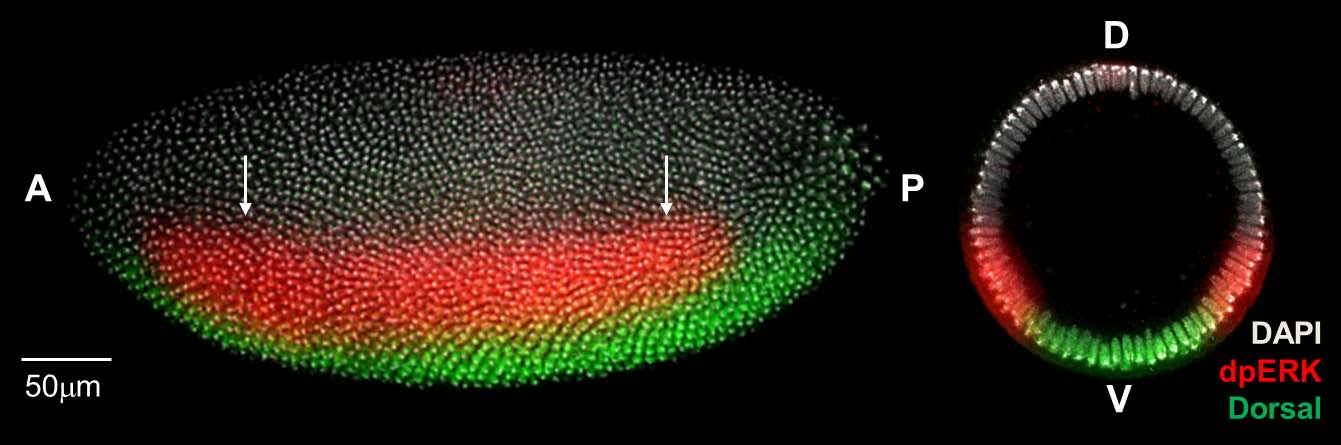
\includegraphics[width=8.4cm]{ap_dv}
\caption{(Left) A lateral view of a {\it Drosophila} embryo stained with DAPI (gray), dpERK (red), and Dorsal (green). Embryo is presented so that the anterior (A) side is to the left and the posterior (P) side is to the right. The arrow indicates the position where the cross-section of an embryo is imaged. (Right) A dorsoventral view of a {\it Drosophila} embryo. The dorsal (D) side is up and the ventral (V) side is down. Images were collected at the focal plane ~18\% from either the anterior or posterior pole of an embryo (arrow in the left image). }
\end{figure}

\begin{figure}
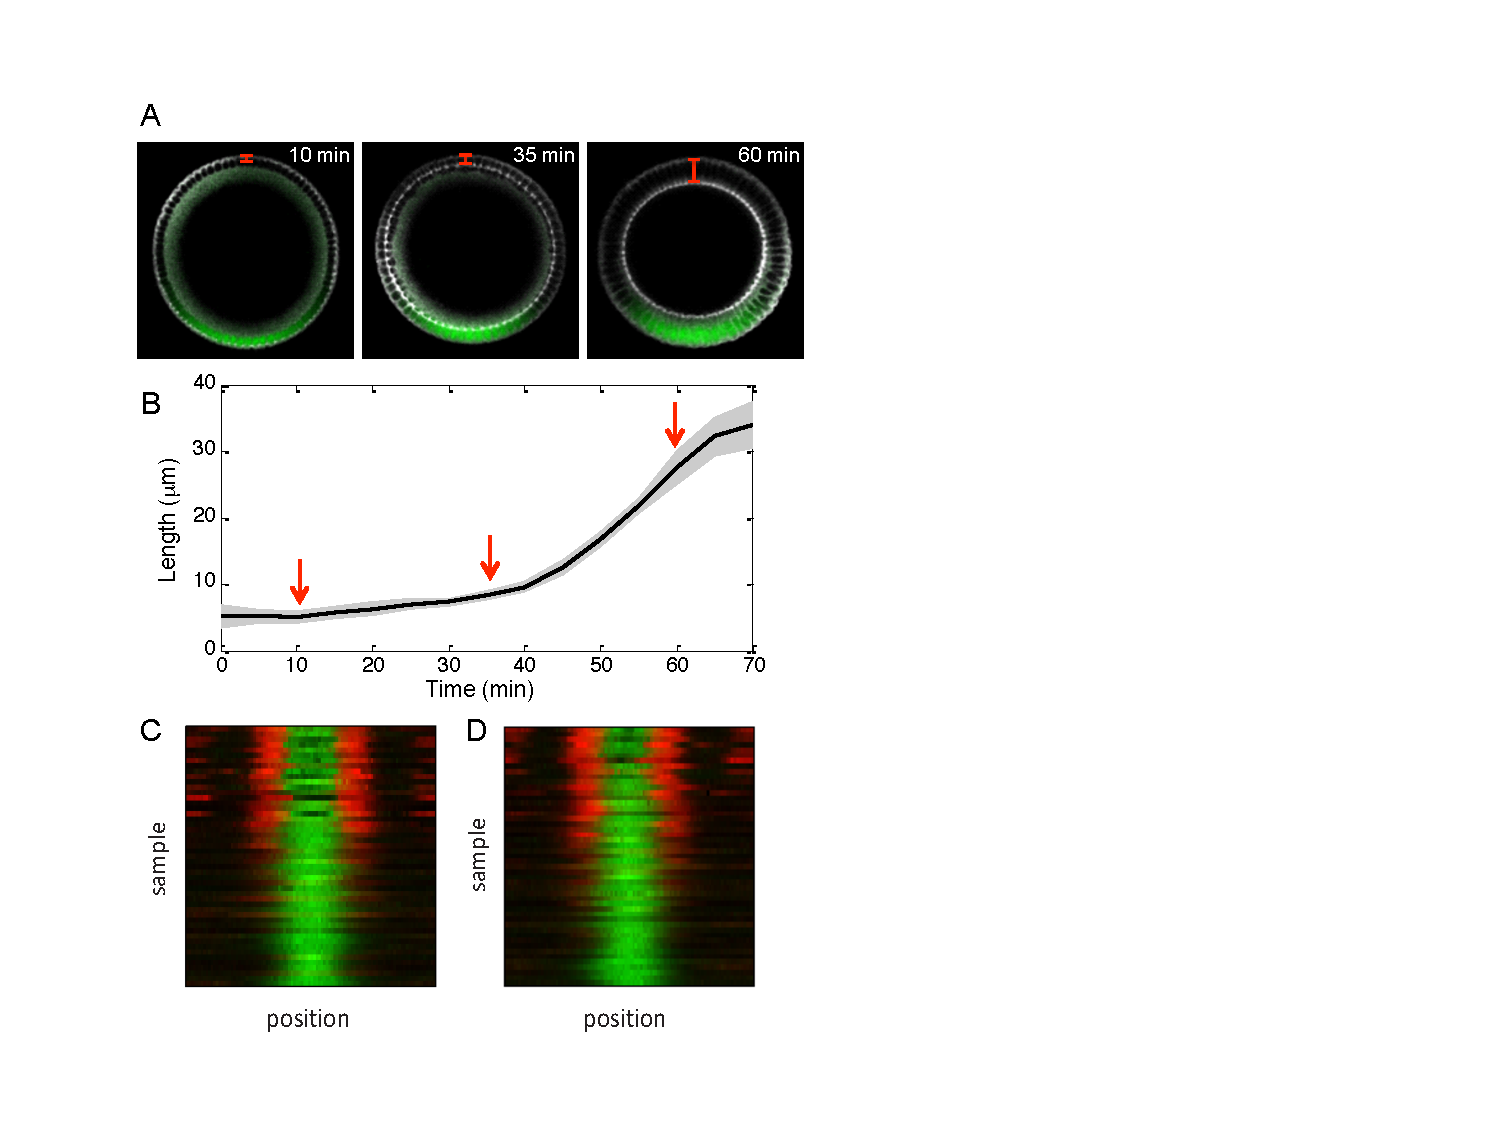
\includegraphics[width=8.4cm, trim=0cm 5.6cm 0cm 0cm, clip]{SI_fig6}
\caption{{\it (A)} Images, stained for membranes (gray) and Dorsal (green) at different times during development. The membrane length is indicated by the red bars. {\it (B)} Membrane length as a function of time. The points corresponding to the images in {\it A} are indicated with arrows.}
\label{fig:membrane_compare}
\end{figure}

\begin{figure}
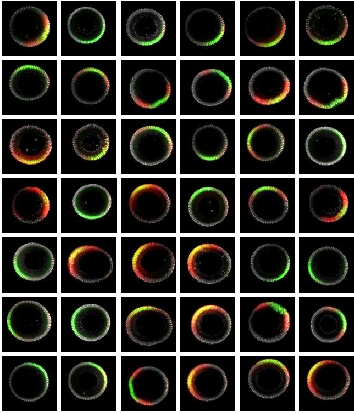
\includegraphics[height=9cm]{raw_data3}
\caption{Images of mutant and wild type {\it Drosophila} embryos during cellularization, used for the analysis in \fig~5. Each image is of a different embryo in a different rotational orientation. Half of the images are of wild type embryos, and half of the images are of mutant embryos.}
\end{figure}

\begin{figure}
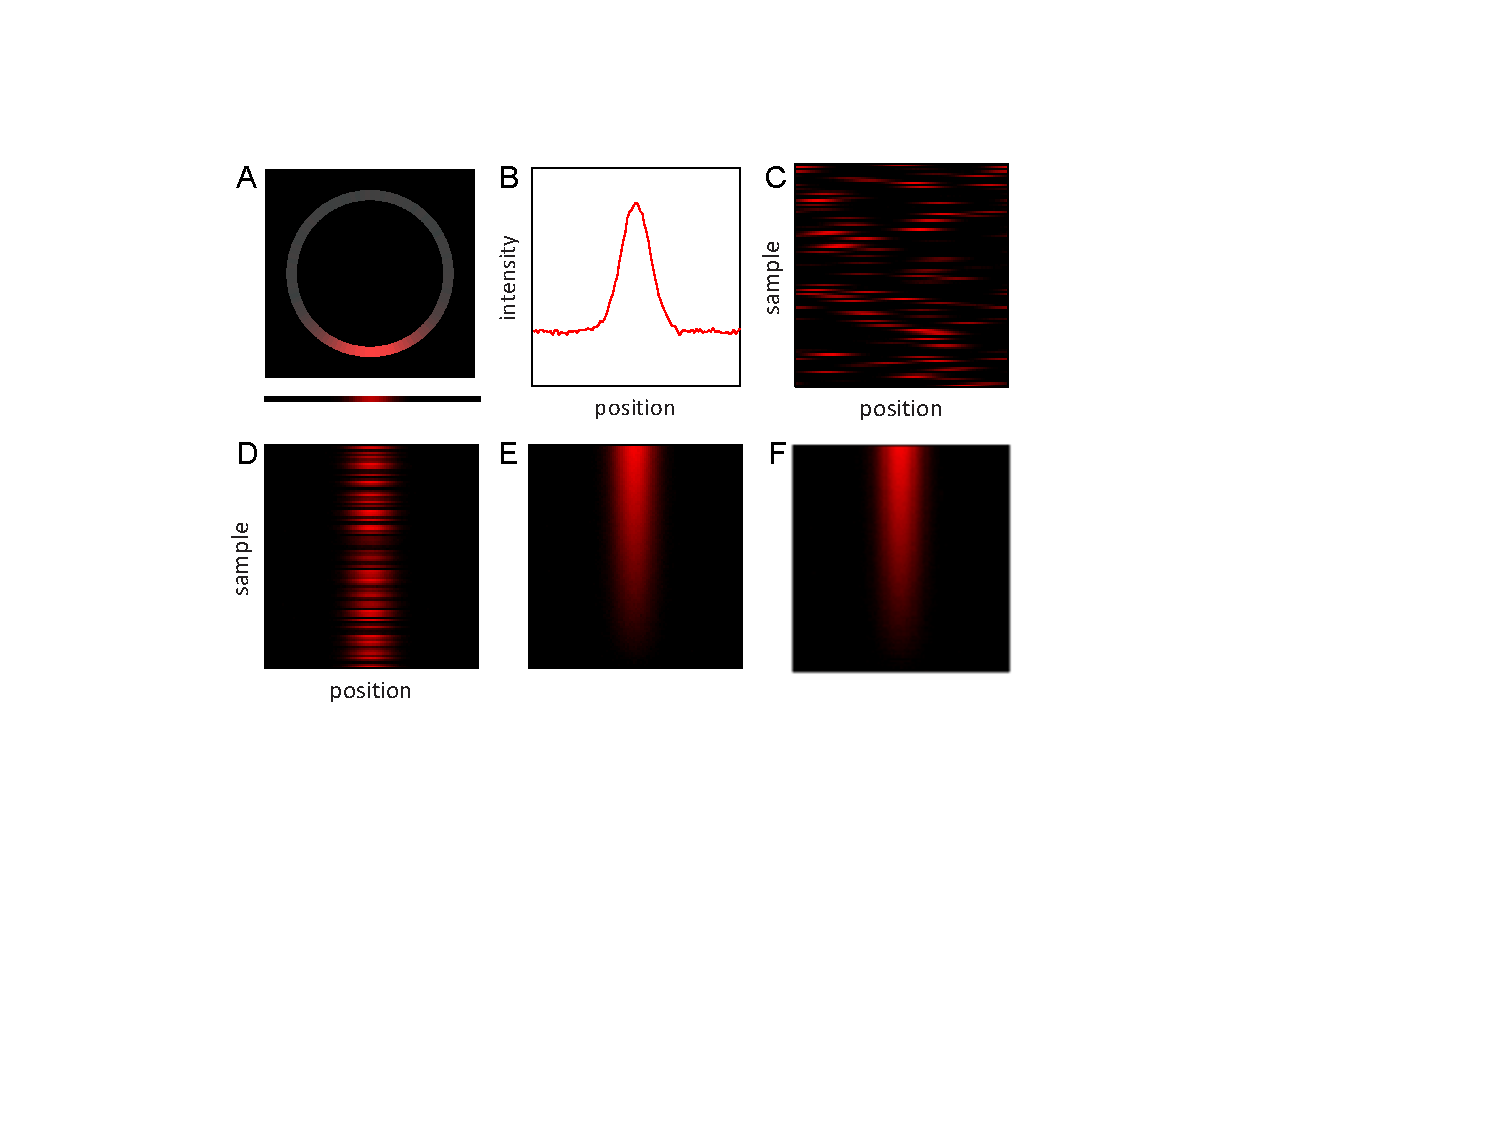
\includegraphics[width=8.4cm]{SI_fig3}
\caption{Synthetic data set used to illustrate the mathematical algorithms. {\it (A)} One-dimensional concentration profile on a ring (top), and the corresponding profile on a line (bottom). {\it (B)} Intensity corresponding to the profile in {\it A}. {\it (C)} An ensemble of concentration profiles, each of the form described in {\it A}. Each row in the array corresponds to a single profile. {\it (D)} The profiles in {\it C}, now registered using angular synchronization. {\it (E)} The profiles in {\it D}, now temporally ordered using diffusion maps. {\it (F)} The profiles in {\it C}, registered and temporally ordered in a single step using vector diffusion maps.}
\label{fig:1d_demo}
%\customlabel{fig:1d_demo}{3}
\customlabel{subfig:1d_example}{\ref{fig:1d_demo}{\it A}}
\customlabel{subfig:1d_intensity}{\ref{fig:1d_demo}{\it B}}
\customlabel{subfig:1d_unaligned_unordered}{\ref{fig:1d_demo}{\it C}}
\customlabel{subfig:1d_aligned_unordered}{\ref{fig:1d_demo}{\it D}}
\customlabel{subfig:1d_aligned_ordered}{\ref{fig:1d_demo}{\it E}}
\customlabel{subfig:1d_aligned_ordered_vdm}{\ref{fig:1d_demo}{\it F}}
\end{figure}

\begin{figure*}
\begin{minipage}{0.2\textwidth}
\centering
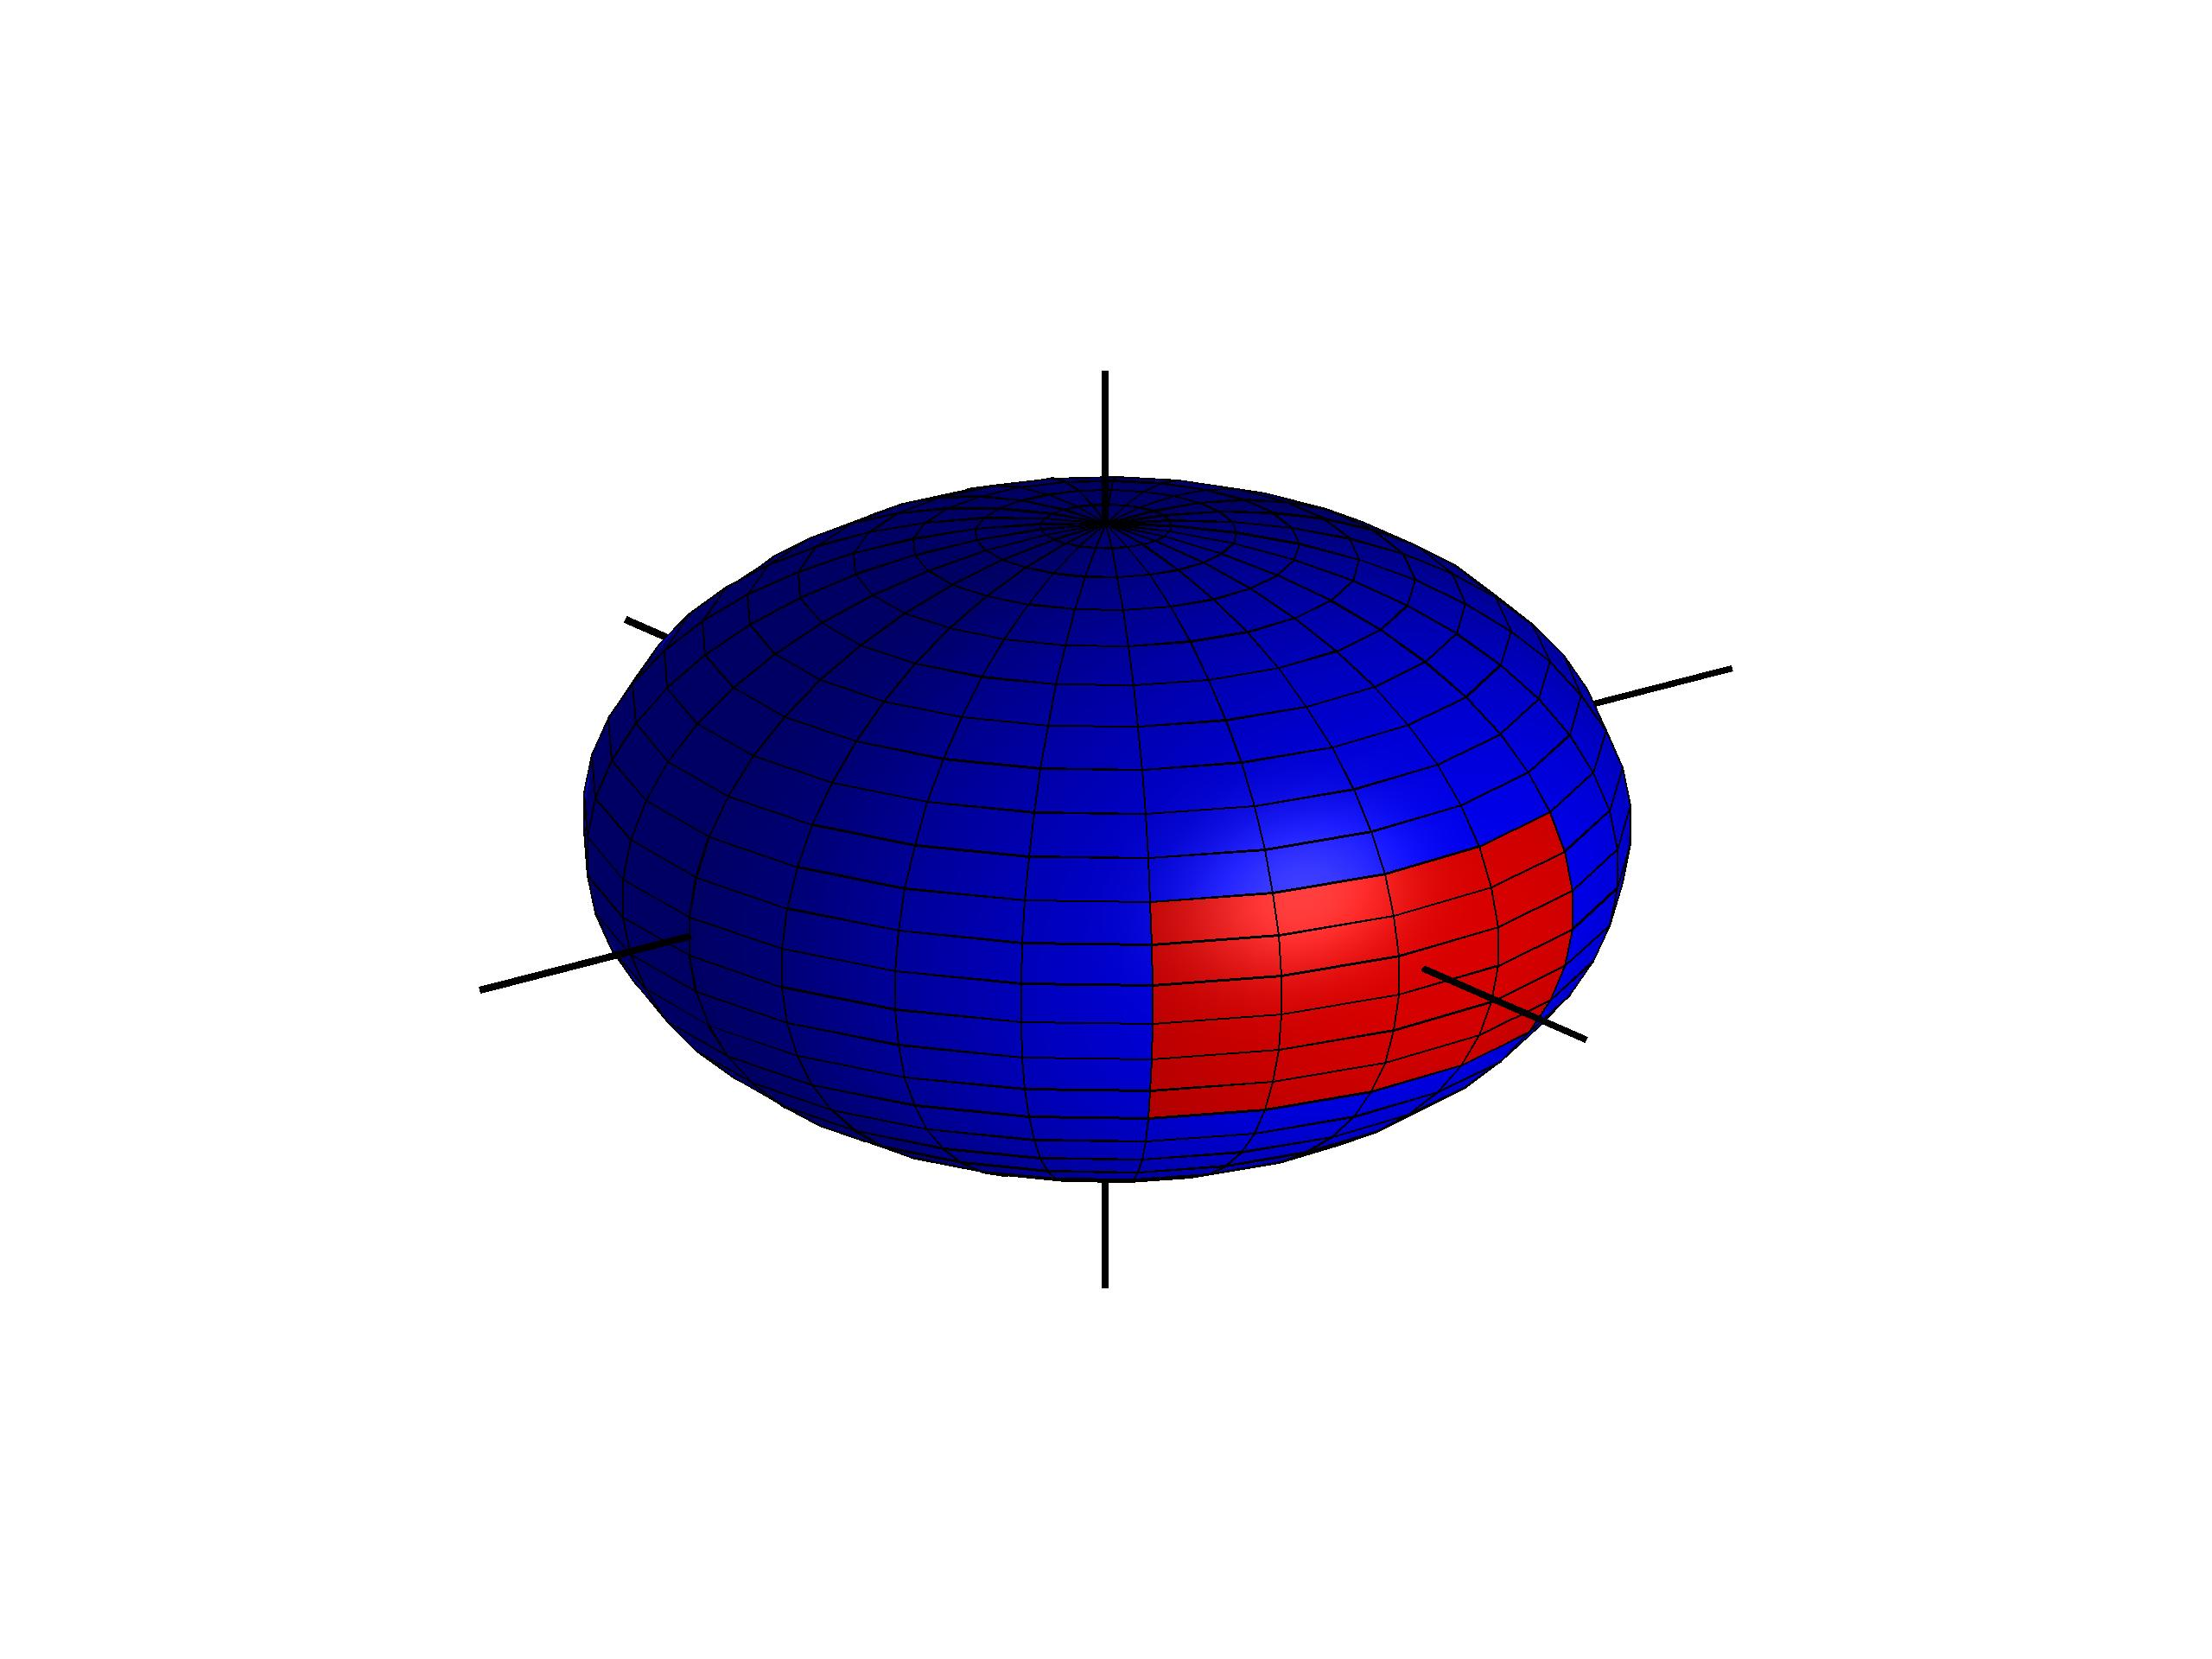
\includegraphics[width=\textwidth]{sphere_1}\\
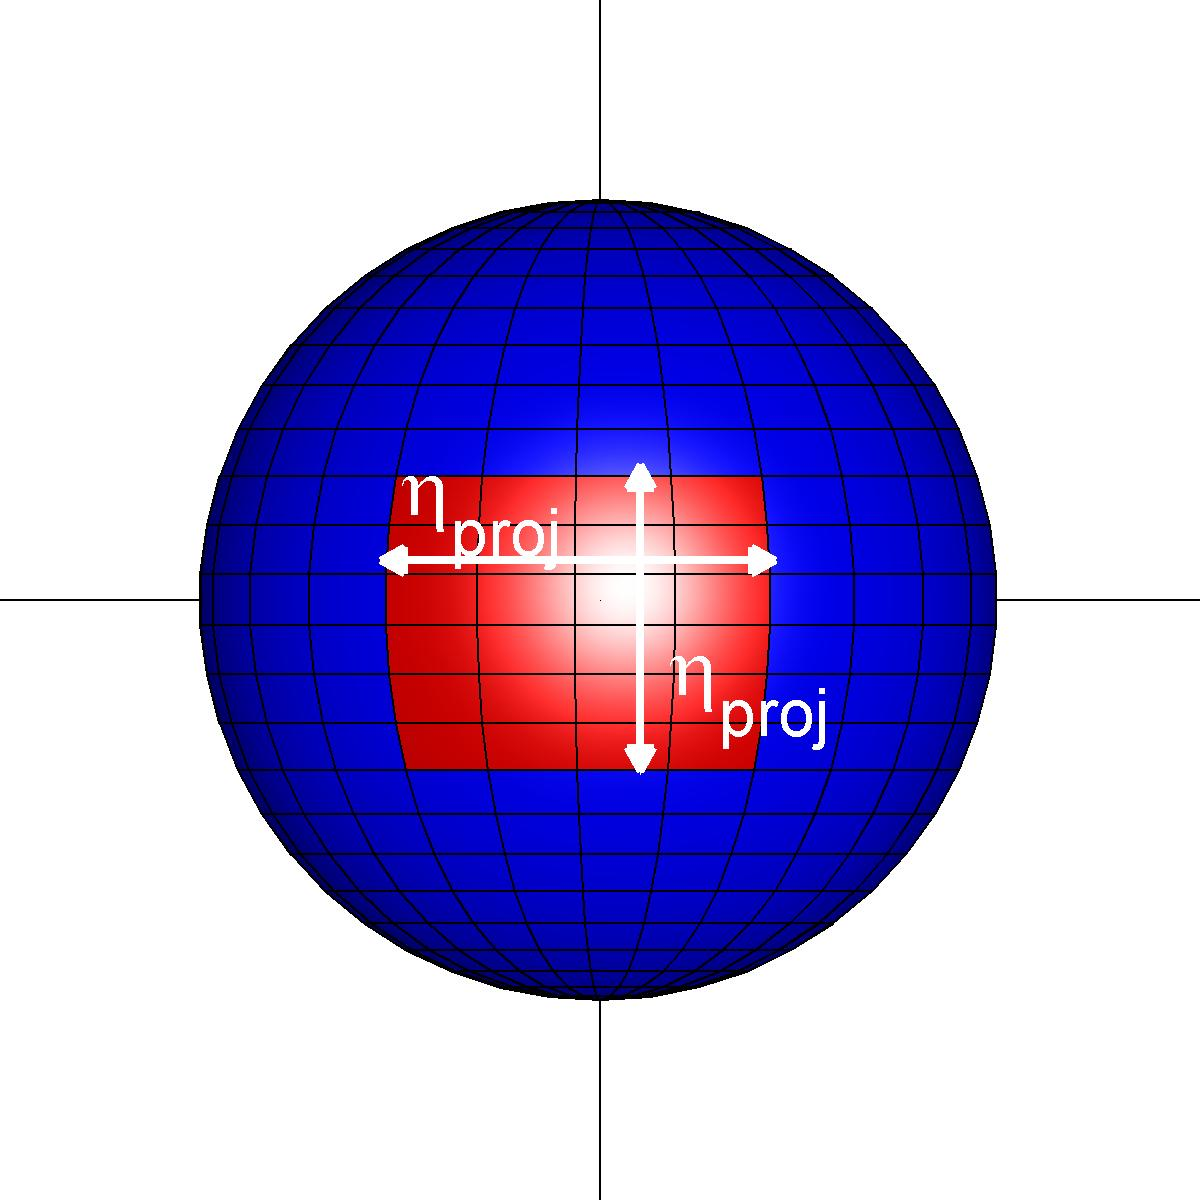
\includegraphics[width=\textwidth]{sphere2_1}\\
\sffamily{A}
\end{minipage}
%
\begin{minipage}{0.2\textwidth}
\centering
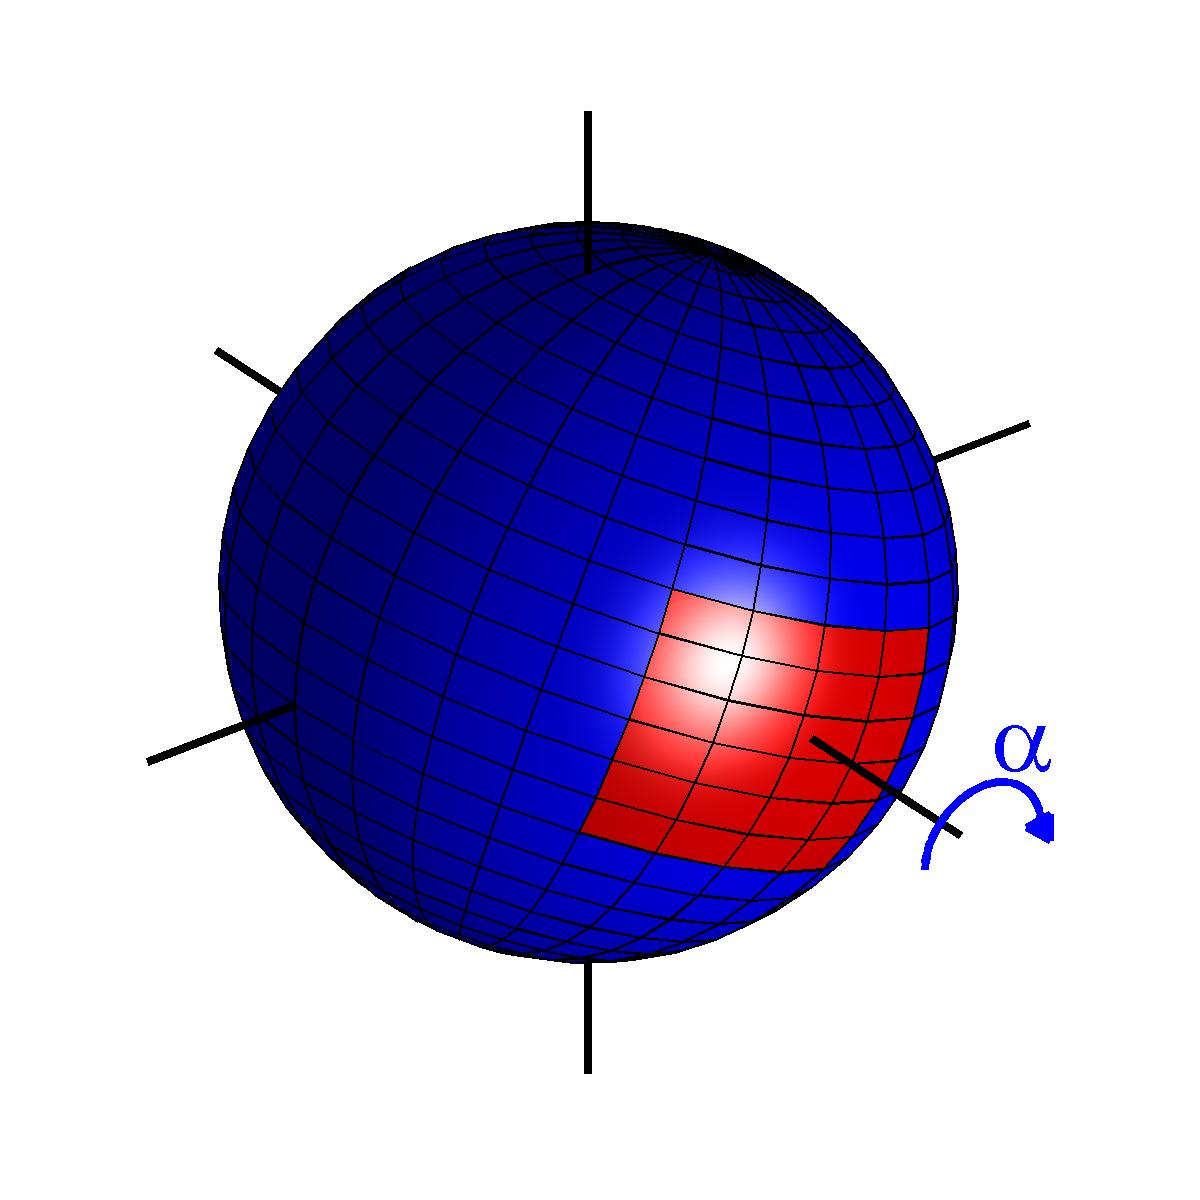
\includegraphics[width=\textwidth]{sphere_2}\\
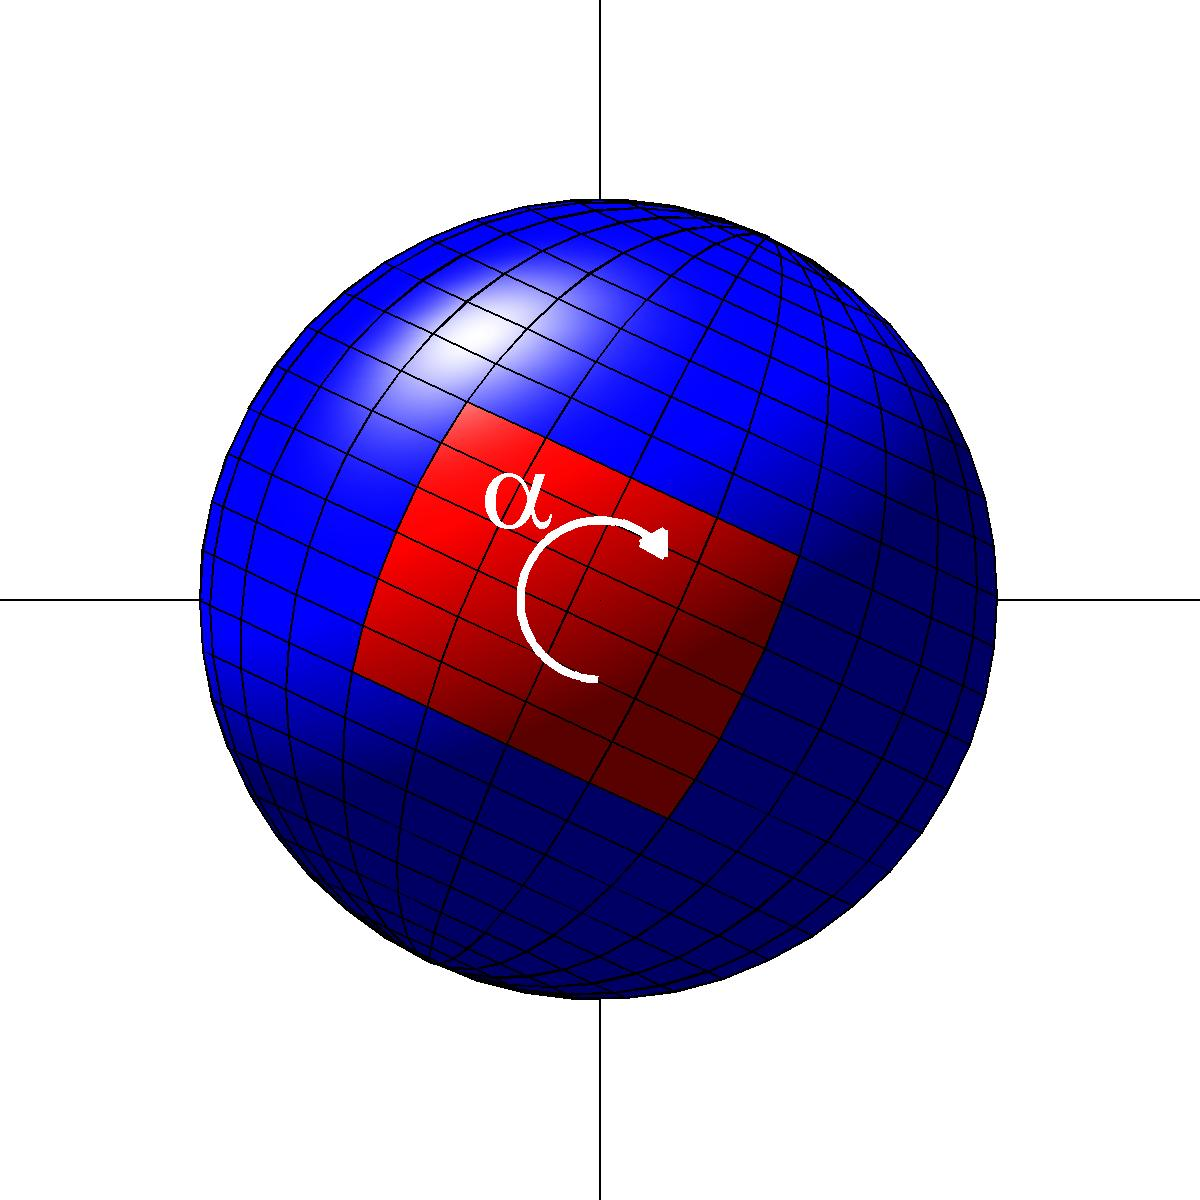
\includegraphics[width=\textwidth]{sphere2_2}\\
\sffamily{B}
\end{minipage}
\begin{minipage}{0.2\textwidth}
\centering
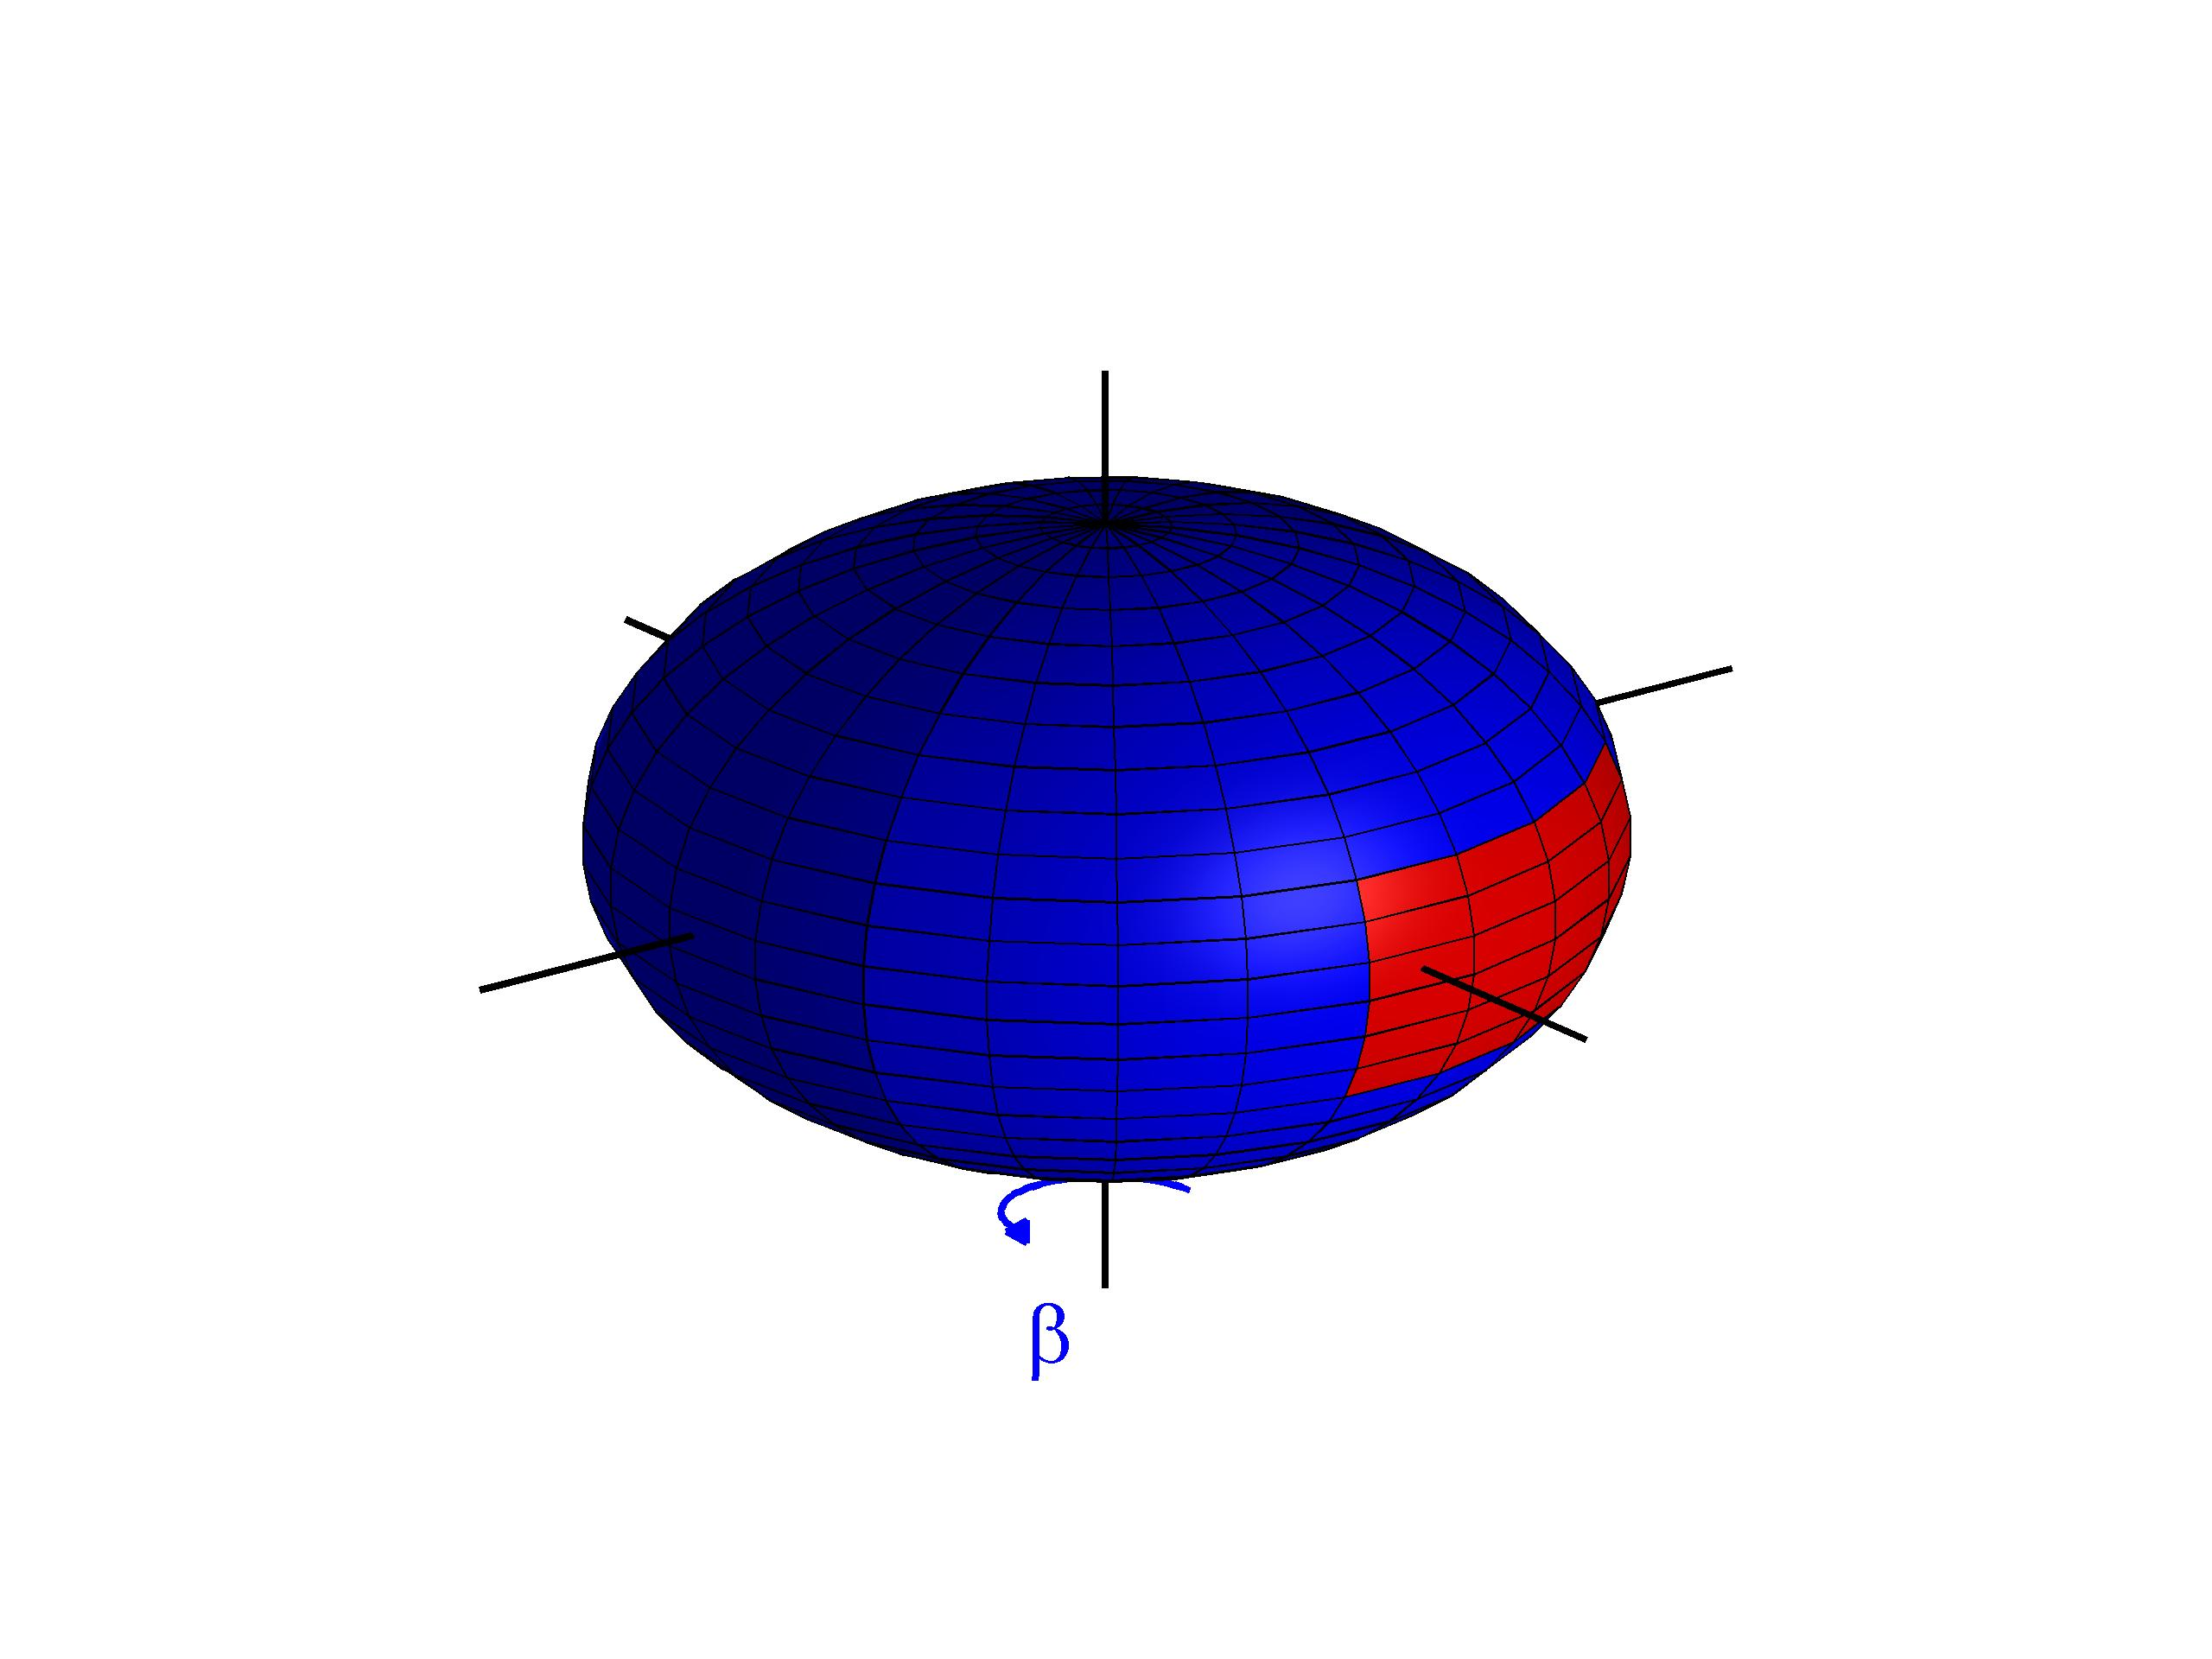
\includegraphics[width=\textwidth]{sphere_3}\\
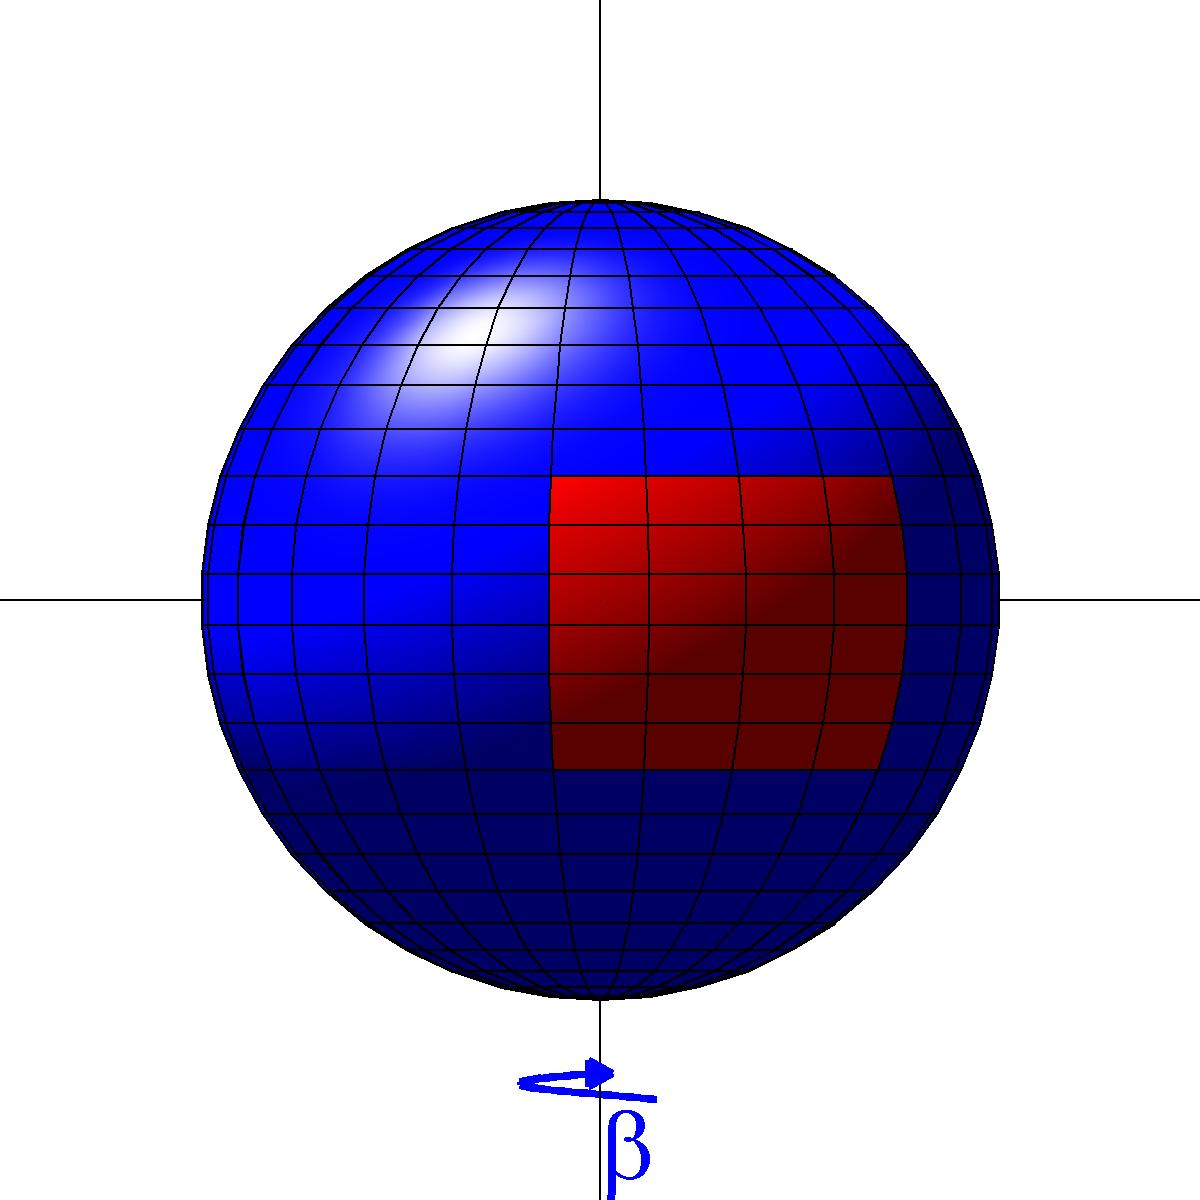
\includegraphics[width=\textwidth]{sphere2_3}\\
\sffamily{C}
\end{minipage}
\begin{minipage}{0.2\textwidth} 
\centering
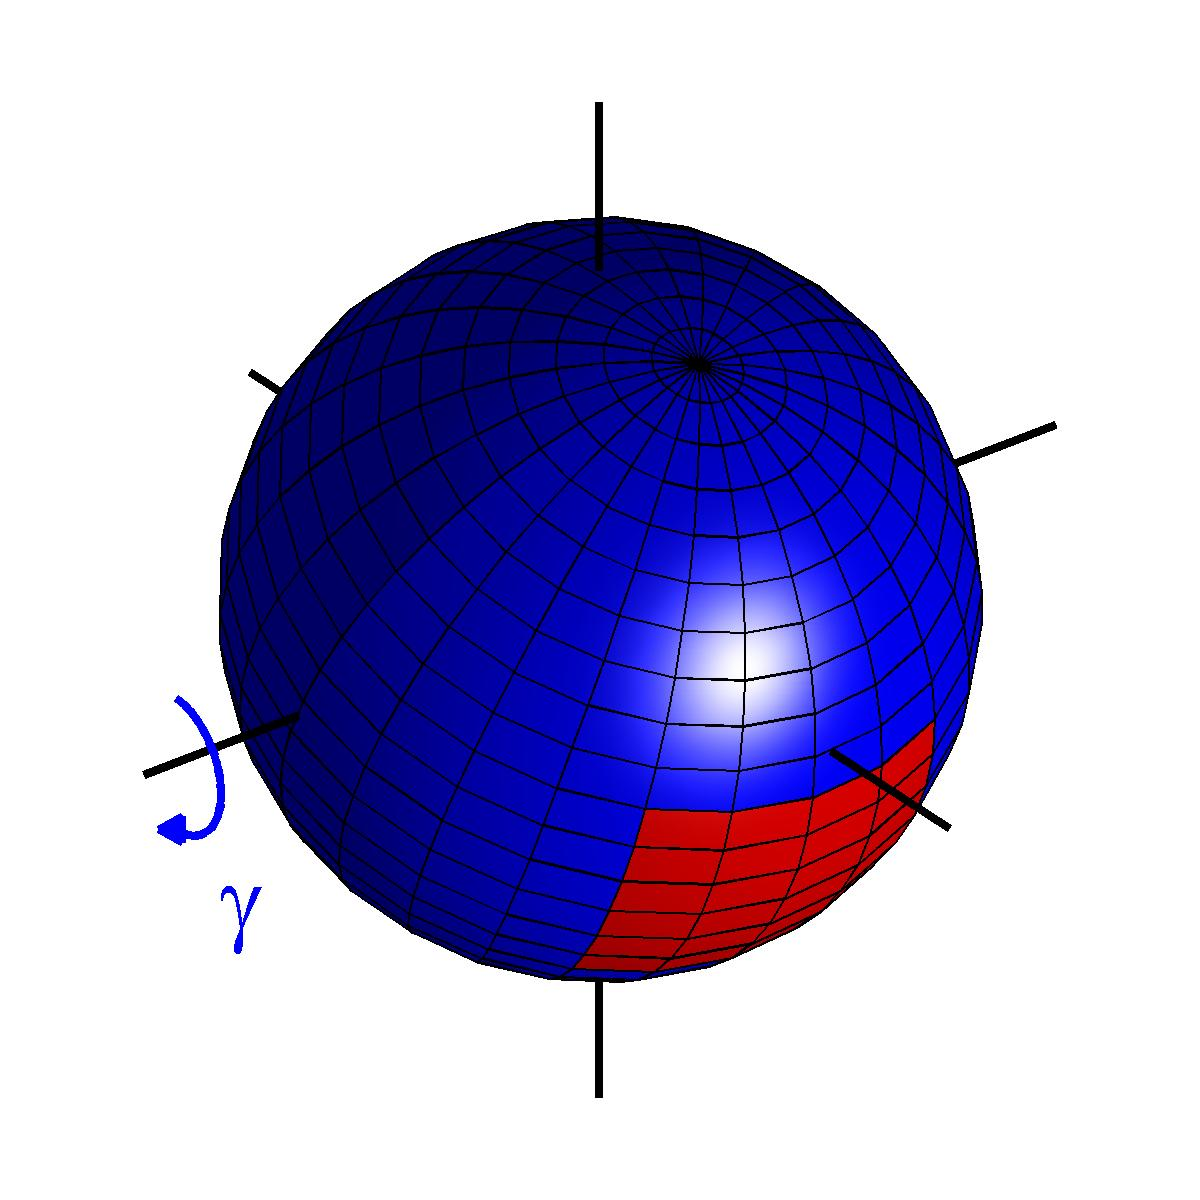
\includegraphics[width=\textwidth]{sphere_4}\\
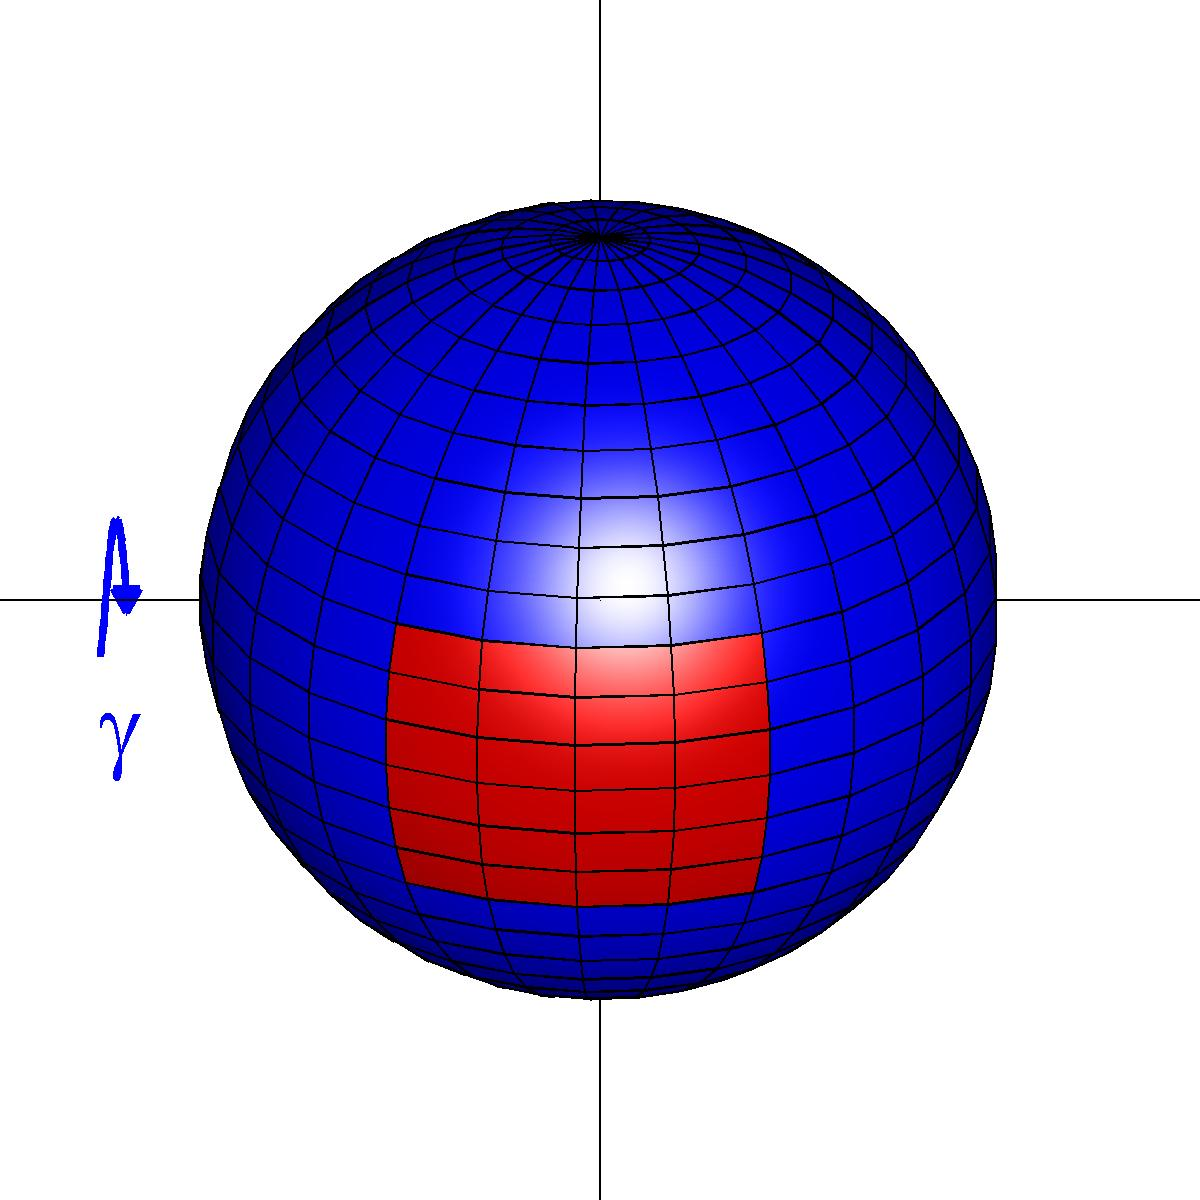
\includegraphics[width=\textwidth]{sphere2_4}\\
\sffamily{D}
\end{minipage}
\caption{Illustration of how rotations in three dimensions correspond to translations and rotations in two dimensions. {\it (A)} The original image (shown in red), projected onto a portion of a sphere. {\it (B)} Rotation around the x-axis (Euler angle $\alpha$) in three dimensions corresponds to rotation of the image. {\it (C)} Rotation around the y-axis (Euler angle $\beta$) in three dimensions corresponds to horizontal translation. {\it (D)} Rotation around the z-axis (Euler angle $\gamma$) in three dimensions corresponds to vertical translation. The top row shows the three-dimensional spheres, and the bottom row shows the (two-dimensional) surface of the sphere in which we are interested.}
\label{fig:SO3_picture}
\end{figure*}

\begin{figure*}
%\raisebox{4.5cm}{\sffamily{A}}
%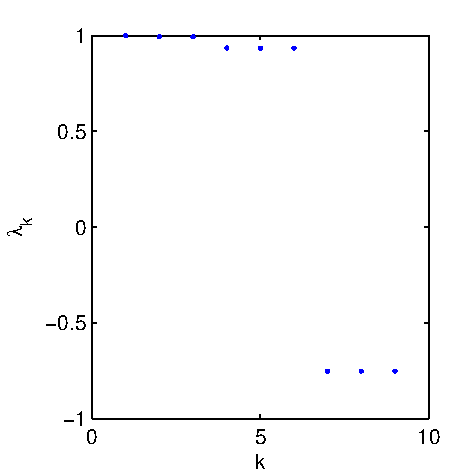
\includegraphics[width=5cm]{data1_evals}
\begin{tikzpicture}
	\node at (0,0) {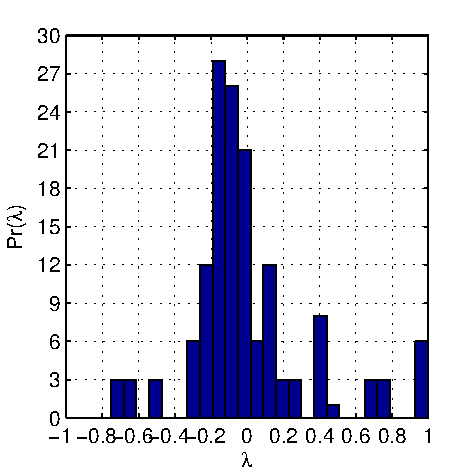
\includegraphics[width=5cm]{data1_evals_dist}};
	\node at (-2.5cm, 2cm) {\sffamily{A}};
	\draw[<->, ultra thick, cyan] (-1.4cm, -1.9cm) -- (1.7cm, -1.9cm);
	\draw[->, ultra thick, red] (1.97cm, -0.5cm) -- (1.97cm, -1cm);
\end{tikzpicture}
%\raisebox{4.5cm}{\sffamily{B}}
%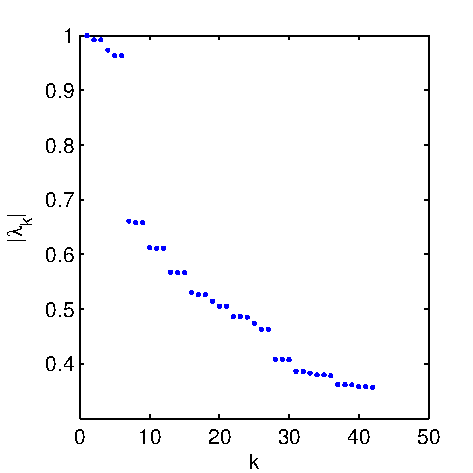
\includegraphics[width=5cm]{data2_evals}
\begin{tikzpicture}
	\node at (0,0) {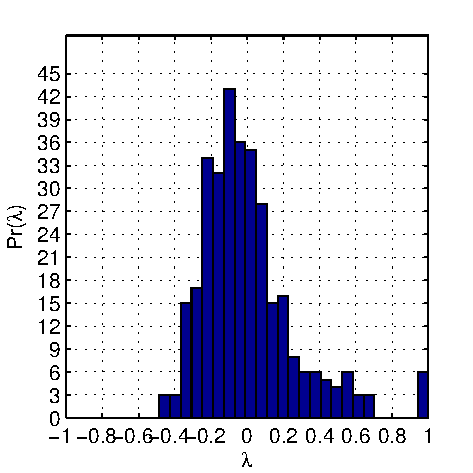
\includegraphics[width=5cm]{data2_evals_dist}};
	\node at (-2.5cm, 2cm) {\sffamily{B}};
	\draw[<->, ultra thick, cyan] (-1.2cm, -1.9cm) -- (1.5cm, -1.9cm);
	\draw[->, ultra thick, red] (1.97, -0.85cm) -- (1.97cm, -1.34cm);
\end{tikzpicture}
%\raisebox{4.5cm}{\sffamily{C}}
%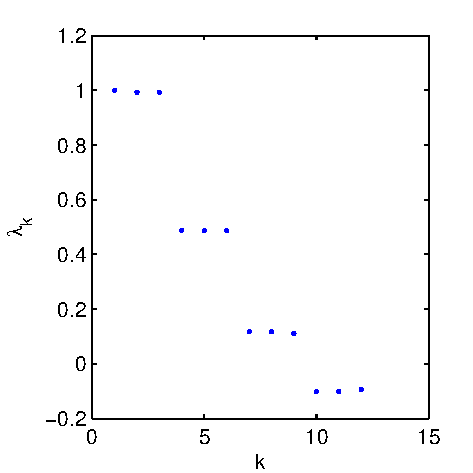
\includegraphics[width=5cm]{data3_evals}
\begin{tikzpicture}
	\node at (0,0) {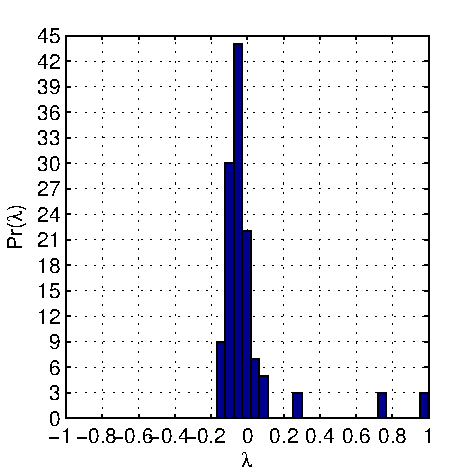
\includegraphics[width=5cm]{data3_evals_dist}};
	\node at (-2.5cm, 2cm) {\sffamily{C}};
	\draw[<->, ultra thick, cyan] (-0.25cm, -1.9cm) -- (0.35cm, -1.9cm);
	\draw[->, ultra thick, red] (1.97, -1.1cm) -- (1.97cm, -1.6cm);
	\draw[->, ultra thick, red] (1.52, -1.1cm) -- (1.52cm, -1.6cm);
	\draw[->, ultra thick, red] (0.64, -1.1cm) -- (0.64cm, -1.6cm);
\end{tikzpicture}
\caption{The histograms of the eigenvalues from vector diffusion maps analysis for the three data sets. 
%
We expect to see an approximately symmetric semicircle distribution centered at 0, which corresponds to noise, and positive eigenvalues separated from the semicircle which correspond to meaningful coordinates. 
%
Each coordinate yields $d=3$ eigenvalues of (approximately) the same magnitude, and the top $d=3$ eigenvalues ($\lambda=1$) correspond to a trivial embedding coordinate.
%
(A) Histogram of eigenvalues from images during cellularization (\fig~3). As expected, we see an approximately symmetric distribution that ranges from $-0.8$ to $0.8$ (indicated by the blue arrow), and $6$ eigenvalues that are outside of this distribution (indicated by the red arrow). $3$ of these eigenvalues correspond to the eigenvector which contains the rotational and translational alignment, and the other $3$ eigenvalues correspond to the first VDM component which uncovers the developmental dynamics, and the then there is an appreciable gap before the third group of eigenvalues.
%
(B) Histogram of eigenvalues from images during gastrulation (\fig~4). We see an approximately symmetric distribution that ranges from $-0.7$ to $0.7$ (indicated by the blue arrow), and $6$ eigenvalues that are outside of this distribution (indicated by the red arrow). $3$ of these eigenvalues correspond to the eigenvector which contains the rotational and translational alignment, and the other $3$ eigenvalues correspond to the first VDM component which uncovers the developmental dynamics.
%
(C) Histogram of eigenvalues from images of mutant and wild type embryos during cellularization (\fig~5).
We see an approximately symmetric distribution that ranges from $-0.2$ to $0.2$ (indicated by the blue arrow), and $9$ eigenvalues that are outside of this distribution (indicated by the red arrows). $3$ of these eigenvalues correspond to the eigenvector which contains the rotational and translational alignment, and the other $2$ eigenvalues correspond to the first two VDM components which uncovers the developmental dynamics of the two genotypes.}
%there is a spectral gap after the first (non-trivial) group of eigenvalues.
%\caption{The eigenvalue spectra from vector diffusion maps analysis for the three data sets. 
%%
%As expected, the eigenvalues appear in groups of 3, as $d=3$ when using vector diffusion maps to register with respect to translations and rotations. 
%%
%(A) Spectrum from images during cellularization (\fig~3). As expected, there is a spectral gap after the first (non-trivial) group of eigenvalues: the first three eigenvalues correspond to the rotational and translational alignment, the second three eigenvalues correspond to the first VDM component which uncovers the developmental dynamics, and the then there is an appreciable gap before the third group of eigenvalues.
%%
%(B) Spectrum from images during gastrulation (\fig~4). Again, 
%there is a spectral gap after the first (non-trivial) group of eigenvalues.
%%
%(C) Spectrum from images of mutant and wild type embryos during cellularization (\fig~5).
%We see a group of three eigenvalues corresponding to the translational and rotational alignments, one group that is clearly significant, and then a second group that, while less important, is still above the level of noise of the subsequent eigenvalues, indicating that two components are necessary to describe the data. }
\label{fig:eval_spectra}
\end{figure*}

\begin{figure}
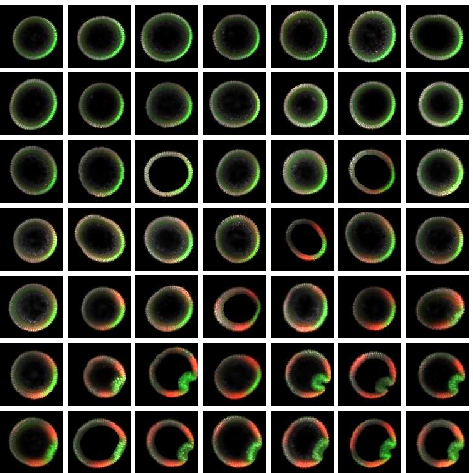
\includegraphics[width=8.7cm]{PCA_ordered}
\caption{Images of embryos during cellularization (from \fig~3), registered using angular synchronization \cite{singer2011angular} and ordered by the first PCA projection coefficient. The recovered dynamics are qualitatively consistent with those recovered by vector diffusion maps. }
\label{fig:PCA_data1}
\end{figure}

\begin{figure*}
\raisebox{5.2cm}{\sffamily{A}}
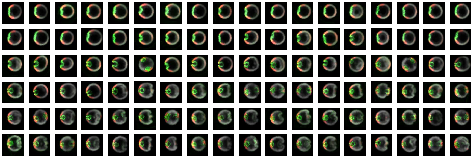
\includegraphics[width=16.8cm]{data2_PCA_ordered}

\raisebox{3.7cm}{\sffamily{B}}
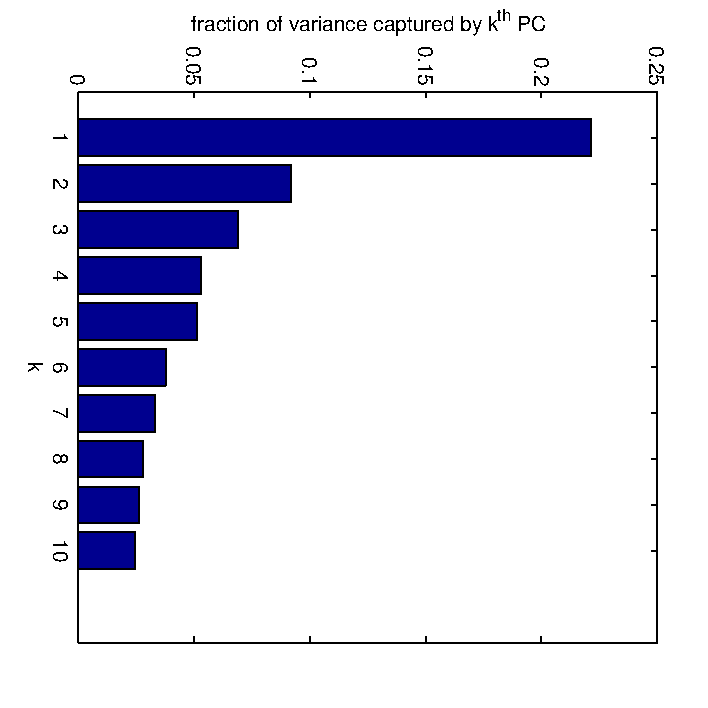
\includegraphics[width=8.4cm]{data2_PCA_variance}
\raisebox{3.7cm}{\sffamily{C}}
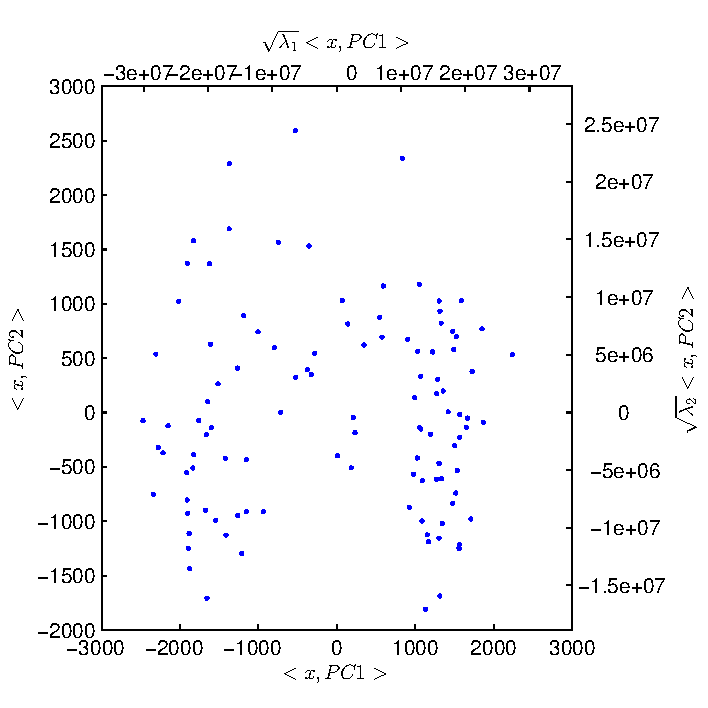
\includegraphics[width=8.4cm]{data2_PCA_proj}

\caption{{\it (A)} Images shown in \fig~4 of the paper, registered using angular synchronization \cite{singer2011angular} and ordered by the first PCA projection coefficient. The recovered ordering is not consistent with the known developmental dynamics. {\it (B)} The fraction of the variance captured by each of the first 10 principal components. Note that components 2--10 have a nonnegligible contribution to the data. {\it (C)} Projection onto the first two principal components.}
\label{fig:PCA_results}
\end{figure*}


\begin{figure*}[t]
\raisebox{7.6cm}{\sffamily{A}}
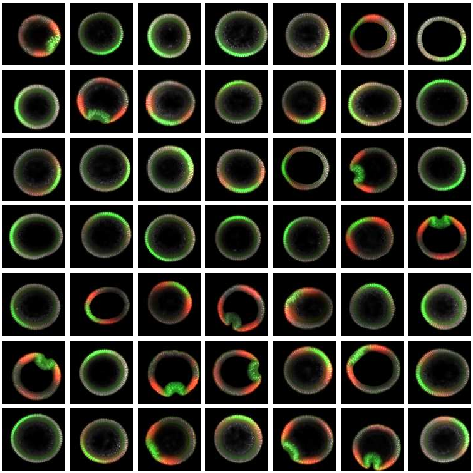
\includegraphics[width=8cm]{raw_data1}
\hfill
\raisebox{7.6cm}{\sffamily{B}}
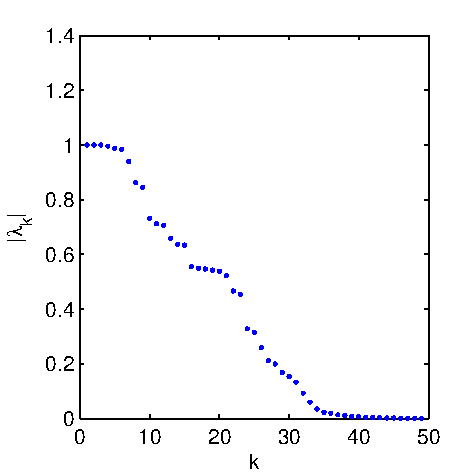
\includegraphics[width=7cm]{FBsPCA_evals}

\raisebox{2.2cm}{\sffamily{C}}
\hspace{-1cm}
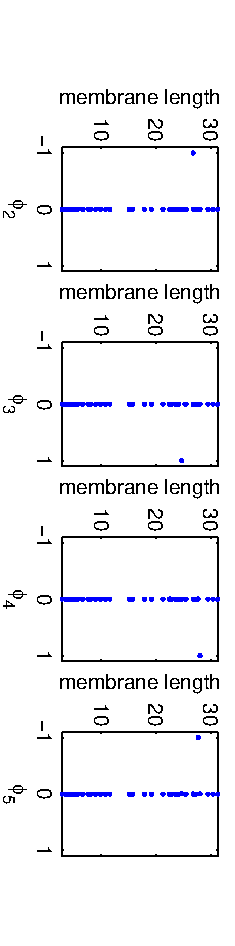
\includegraphics[width=4cm, angle=90]{FBsPCA_dmaps}
\caption{I computed the FBsPCA basis for the set of images (separately for the red and green signals).
%
I then computed the bispectrum coefficients for each image expanded in the FBsPCA basis, and used these coefficients in a DMAPS calculation.
%
The results are shown below.
%
However, because the bispectrum is not stable to deformations, it does not seem to be able to identify neighboring images.
%
(A) Images used for FBsPCA. (B) Eigenvalue spectrum from dmaps, using bispectrum coefficients. There is no spectral gap after the first component, as would be expected for this particular data set. (C) First 4 diffusion maps variables, computed from the bispectrum coefficeints, plotted against the membrane thickness. Note there is no appreciable correlation: each dmaps variable simply selects one image from the data set as ``abnormal''.}
\end{figure*}


\end{document}